%% Chapter 2 — 가상화 원리와 클라우드 컴퓨팅
\setcounter{chapter}{1}
\chapter{가상화 원리와 클라우드 컴퓨팅}
\chaptersubtitle{"GPU VM을 빌릴" 때 실제로 일어나는 일 — CPU 모드부터 microVM과 MIG까지}

\begin{calloutbox}{tbbblue}{tbbbluefill}
{\normalsize\bfseries\color{tbbblue}학습 목표}\par\vspace{3pt}
\begin{tbbitemize}
  \item 임대한 클라우드 VM을 \code{dmidecode}, \code{systemd-detect-virt}, \code{kvm-clock}로 심문해 물리적으로 존재하지 않는다는 증거를 읽고, 산업이 이 환상을 계속 다시 만드는 이유를 설명하는 60년의 사용률 역사(수백만 달러짜리 메인프레임 → 2000년대의 빈 서버 → EC2의 시간당 \$0.10)를 재구성한다.
  \item Popek과 Goldberg가 제시한 가상 머신 모니터의 세 요구 사항을 말하고, 고전적 x86이 이를 충족하지 못한 이유와 2005년까지 산업을 지탱한 두 소프트웨어 우회책인 바이너리 변환과 반가상화를 설명한다.
  \item VMX root/non-root 모드, VMCS, VM exit, EPT/NPT를 포함한 하드웨어 지원 가상화를 설명하고, "exit의 횟수와 비용"이라는 관점으로 가상화 성능을 분석한다.
  \item KVM, QEMU, virtio가 Linux에서 VM 실행 작업을 어떻게 나누는지, 반가상 장치가 에뮬레이션 장치보다 빠른 이유를 설명한다.
  \item 프로세스, 컨테이너, gVisor, microVM, 완전한 VM을 격리 스펙트럼 위에 놓고, AWS가 Lambda를 위해 Firecracker를 만든 이유를 포함해 주어진 멀티테넌트 워크로드에 어느 지점이 맞는지 논증한다.
  \item GPU가 워크로드에 도달하는 세 방식인 PCIe 패스스루, vGPU/시간 분할, MIG를 비교하고 성능 격리와 비용에 미치는 영향을 설명한다.
  \item 과금 안전장치를 가장 먼저 마련한 뒤 첫 클라우드 GPU VM을 시작하고, CPU와 GPU 추론을 벤치마크하며, 안전하게 종료한다.
\end{tbbitemize}
\end{calloutbox}

\vspace{5.0pt}

\begin{calloutbox}{tbbteal}{tbbtealfill}
{\normalsize\bfseries\color{tbbteal}핵심 용어}\par\vspace{3pt}
시분할(CP-67 / VM) · 서버 난립 · 사용률 · 하이퍼바이저 / VMM · Type 1 대 Type 2 · 트랩 후 에뮬레이션 · 민감 명령어 대 특권 명령어 · 바이너리 변환 · 반가상화 · VT-x / AMD-V · VMX root/non-root · VMCS · VM exit · EPT / NPT · KVM · QEMU · vCPU · 스틸 타임 · virtio · virtqueue · vhost · SR-IOV · IOMMU (VT-d) · microVM · Firecracker · gVisor · Kata Containers · PCIe 패스스루(VFIO) · vGPU · 시간 분할 · MPS · MIG
\end{calloutbox}

\vspace{5.0pt}

\begin{calloutbox}{tbblightgray}{tbbboxfill}
{\normalsize\bfseries\color{tbbink}장 구성}\par\vspace{3pt}
\textbf{2.1} 빌린 머신은 존재하지 않는다    \textbf{2.2} 하이퍼바이저와 트래핑 문제    \textbf{2.3} 하드웨어 지원 가상화: VT-x, VMCS, EPT    \textbf{2.4} KVM, QEMU, virtio: 클라우드의 하이퍼바이저가 된 Linux    \textbf{2.5} VM은 얼마나 작아질 수 있는가? microVM과 격리 스펙트럼    \textbf{2.6} 클라우드의 GPU: 인스턴스, 패스스루, 공유    \textbf{2.7} 실습: 첫 클라우드 GPU를 안전하게 사용하기 — 이후 요약, 연습문제, 더 읽을거리로 이어진다.
\end{calloutbox}

\section{빌린 머신은 존재하지 않는다}

이번 주 어느 시점에 \textbf{Launch instance}라고 쓰인 버튼을 누르고 40초가량 기다린 뒤 "자신의" 머신에 ssh로 접속할 것이다. 그 머신에는 호스트 이름, CPU, 메모리, 디스크, 그리고 이 과정에서 처음으로 GPU까지 있다. 재부팅할 수도 있고 망가뜨릴 수도 있다. 모든 면에서 자기 소유의 컴퓨터처럼 동작한다.

이 장에서 풀어낼 불편한 진실은 \textbf{그 컴퓨터가 존재하지 않는다}는 것이다. 버튼을 눌렀을 때 누군가 서버를 랙에 꽂은 것이 아니다. 데이터 센터 어딘가에는 128개 코어와 2테라바이트 RAM을 갖췄을 법한 거대한 물리 머신이 있다. 그 위에서 이와 같은 게스트 수십 개가 나란히 실행되며, 각자 하드웨어를 소유한다고 믿는다. 이 환상을 유지하는 소프트웨어가 \textbf{하이퍼바이저}, 또는 \textbf{가상 머신 모니터(VMM)}다. 환상 자체는 \textbf{가상 머신(VM)}으로, 물리 컴퓨터를 충실하고 격리된 소프트웨어 정의 사본으로 만든 것이다.

\subsection*{사례 A: 머신을 심문하다}

강한 주장에는 증거가 필요하다. 이 주장은 명령 여섯 개만으로 스스로 유죄를 입증한다. 머신은 파일에 자신의 본성을 기록해 두고 있으므로 물어보기만 하면 된다.

\begin{terminalbox}
\begin{Verbatim}[breaklines=true,breakanywhere=true,fontsize=\small,formatcom=\color{tbbtermfg},codes=\tbbcodeactive]
$ ssh ubuntu@203.0.113.7            # "your" machine, forty seconds old
$ sudo dmidecode -s system-manufacturer
Amazon EC2                          # the "manufacturer" is a retailer
$ sudo dmidecode -s system-product-name
g4dn.xlarge                         # the "model number" is a price tag
$ systemd-detect-virt
kvm                                 # the OS knows. it has always known.
$ lscpu | grep Hypervisor
Hypervisor vendor:   KVM
$ cat /sys/devices/system/clocksource/clocksource0/current_clocksource
kvm-clock                           # even TIME arrives via the hypervisor
$ nvidia-smi -L
GPU 0: Tesla T4 (UUID: GPU-8f61c81e...)   # and yet THIS is physically real
\end{Verbatim}
\end{terminalbox}
\figcaption{사례 2-A  임대한 머신을 심문한 결과. 펌웨어 문자열, 가상화 감지기, CPU 플래그, 시계까지 모든 계층이 이 컴퓨터가 소프트웨어임을 증언한다. 마지막 줄만은 예외이며, 2.6절에서 설명한다.}

자백을 한 줄씩 읽어 보자. 노트북이라면 \textit{LENOVO}와 모델 번호가 들어갈 DMI 펌웨어 문자열 필드에 소매업체 이름과 과금 SKU가 들어 있다. 하이퍼바이저가 작성했고 \textit{그 부분}까지 거짓말할 이유는 없었기 때문이다. \code{systemd-detect-virt}가 특별한 묘기를 부리는 것도 아니다. 게스트는 단순히 물어볼 수 있다(하이퍼바이저용으로 예약된 \code{CPUID} 리프이며, 2.3절에서 누가 답하는지 설명한다). 스케줄에서 밀려난 게스트는 혼자 정확한 시간을 유지할 수 없으므로 시계조차 반가상 서비스다. \code{kvm-clock}과 사촌인 \textit{스틸 타임}은 p99를 달고 2.4절에 다시 등장한다. 그런데 마지막 줄은 이 패턴을 거부한다. 디스크도 가상이고 NIC도 가상이며 시간 자체도 가상이지만, T4는 \textbf{통째로 패스스루된 실제 카드}다. 가장 비싼 구성 요소 하나만 빼고 전부 가짜인 머신은 기묘한 산물이다. 2.6절을 마치면 산업이 정확히 왜 이런 식으로 만드는지 알게 된다.

\subsection*{사례 B: 텅 빈 머신들}

애초에 이 환상은 왜 존재할까? 우아함 때문이 아니라 \textbf{돈} 때문이다. 50년 간격으로 두 번이나 그랬다. 이 과정이 이야기의 3막 안에 자리하기 때문에 세 문단을 들여 살펴볼 가치가 있다.

\textbf{1막: 머신 가격이 수백만 달러다(1960년대).} 당시 메인프레임은 수백만 달러였으며, 제작자가 처음 의도한 대로 한 번에 작업 하나만 실행하면 사람이 테이프를 바꾸는 작업 사이에 놀고 있었다. \textit{귀중한 머신 하나를 여러 사용자가 나눠 써야 한다}는 경제적 압력이 시분할을 낳았다. IBM Cambridge 연구소에서는 더 기묘하고 오래가는 산물인 \textbf{CP-67 (1967)}이 탄생했다. 사용자에게 로그인 세션이 아니라 \textit{각자의 완전한 System/360 시뮬레이션}을 제공하고, 그 안에서 사용자별 단일 사용자 OS를 실행하는 소프트웨어였다. 가상화는 클라우드를 위해 발명된 것이 아니다. 하드웨어가 비싸면서도 놀고 있었기 때문에 탄생했으며, UNIX보다도 오래되었다.

\textbf{2막: 머신이 텅 비어 있다(2000년대).} 시간을 빠르게 돌려 보자. 서버가 저렴해지자 기업은 애플리케이션마다 한 대씩 구매했다. 관리 편의도 이유였고, "메일 서버와 데이터베이스가 \textit{반드시} 싸울 것"이라는 미신도 한몫했다. 그 결과 \textbf{서버 난립}이 벌어졌다. 베이지색 상자가 랙을 가득 채웠고, 당시 조사에서 일반적인 사용률은 \textbf{5–15\%}였다. 사실상 기업 데이터 센터는 각각 전력과 냉각 비용을 태우는 유휴 CPU 창고였다. 2.2절에서 설명하듯 기술적 이유로 가상화를 거부하던 x86에 VMware가 1960년대의 묘수를 되살렸다(1999–2001). 대부분 놀고 있는 머신 10대를 한 대로 접는 \textit{통합}은 스스로 가치를 입증했다. 투자 수익률 논리는 말 그대로 "전기 요금 청구서 아홉 장을 없앤다"였다.

\textbf{3막: 계량기(2006년).} 2006년 8월 25일, Amazon은 Elastic Compute Cloud라는 서비스의 베타를 열었다. API로 빌리는 가상 머신이며 소형 인스턴스 가격은 \textbf{\$0.10 per hour}였다. 중요한 단어는 \textit{클라우드}가 아니라 \textit{시간}이었다. 할당이 소프트웨어 작업(이 장의 주제)이 되었으므로 계산 자원을 전기처럼 계량할 수 있었다. 조달도, 랙 설치도, 최소 사용량도 필요 없었다. 제1장에서 배운 모든 경제 구조, 즉 GPU 시간당 가격, 토큰당 API, 서버리스 과금, 사례 1-B의 \$779 교훈까지 모두 그 계량기에서 내려왔다. 그리고 이 이야기를 우리 이야기로 만드는 대칭이 있다. \textbf{GPU가 지금 다시 1막을 살고 있다.} H100은 이번 10년의 수백만 달러짜리 메인프레임이다. 터무니없이 비싸고 만성적으로 충분히 공유되지 않는다. 2.6절의 패스스루 → 시간 분할 → MIG는 CPU가 세 막에 걸쳐 밟은 여정(독점 사용 → 소프트웨어 공유 → 하드웨어 파티션)을 실리콘에서 다시 재생한다. 아키텍처에는 운율이 있고, 이 장은 그 운율 체계를 가르친다.

제1장에서는 "GPU VM을 빌린다"는 말을 믿고 받아들였다. 이 장에서는 상자를 연다. 안의 메커니즘은 세부 사항이 아니라 이 과정의 모든 주제가 서 있는 기반이기 때문이다. 먼저 이유 네 가지를 살펴보자.

\subsection*{클라우드가 가상화 위에 구축된 이유}

\textbf{첫째: 사용률의 경제성.} 제1장에서 AI 인프라 비용의 핵심 문제는 비싼 하드웨어가 놀고 있는 것이라고 배웠다. 고객 한 명에게 통째로 판매한 물리 서버는 그 고객이 쉴 때 함께 논다. 물리 서버를 가상 머신으로 나누면 부하의 고점과 저점이 엇갈리는 여러 테넌트를 수용할 수 있다. 공급자는 같은 실리콘을 여러 번 판매하고, 고객이 원하는 만큼 작은 조각을 원하는 시간만큼 제공할 수 있다. 제1장 표 전체의 경제적 전제인 시간당 과금은 할당이 소프트웨어 작업이기 때문에 가능하다.

\textbf{둘째: 낯선 사용자 사이의 격리.} VM은 절대 만날 일이 없는, 어쩌면 경쟁사일 수도 있는 테넌트와 물리 머신을 공유한다. 하이퍼바이저는 다른 테넌트가 내 메모리를 읽거나 CPU 몫을 소진하거나 커널을 충돌시키지 못하도록 보장하는 심판이다. 그 심판이 얼마나 강력하며 성능 비용은 얼마인지가 이 장을 관통하는 주제다. 워크로드가 "빌린 서버"에서 "200 ms 동안만 사는 서버리스 함수"로 작아지면 답이 달라지므로 2.5절 전체가 이 문제를 다룬다.

\textbf{셋째: 탄력성은 소프트웨어 호출 한 번이면 된다.} 제1장에서 추론 부하는 급증하며 해결책은 탄력적 스케일링이라고 배웠다. "머신 생성"이 하드웨어를 랙에 꽂는 일이 아니라 프로세스와 비슷한 소프트웨어 객체를 만드는 일이므로 탄력성이 물리적으로 가능하다. 12주 차에 오토스케일링을 배울 때 모든 수평 확장 이벤트의 바닥에는 이 장에서 설명하는 할당, 부팅, 로드, 서빙의 순서가 있다. 이 순서에 걸리는 시간이 \textbf{콜드 스타트}다. 하한은 가상화 기술이 정하며, AWS가 Lambda를 실용화하려고 새로운 VM인 Firecracker(2.5절)를 발명해야 했던 이유다.

\textbf{넷째: 서버군은 이기종이지만 VM은 그렇지 않다.} 공급자는 여러 세대의 하드웨어를 나란히 운영한다. 가상화 계층은 이 동물원을 안정적인 인스턴스 유형으로 정규화한다. 공급자는 게스트가 실행되는 동안에도 호스트를 마이그레이션하고 비우고 패치할 수 있으며, 사용자는 머신 전체를 파일로 스냅숏할 수 있다. 하드웨어 프로젝트가 될 작업이 API 호출로 바뀐다.

\subsection*{AI 서빙 엔지니어가 내부 구조를 알아야 하는 이유}

VMCS가 무엇인지 모르고도 수년 동안 클라우드를 사용할 수 있다. 그러나 이 과정은 의존하는 추상화 아래로 내려가겠다고 약속했고, 이 계층을 방문하면 특히 큰 보상을 얻는다.

\begin{tbbitemize}
  \item \textbf{p99의 뿌리가 이곳까지 내려온다.} vCPU는 호스트가 스케줄링하는 스레드다(2.4절). 과도하게 판매된 호스트에서 게스트는 "스틸 타임"을 겪는다. 애플리케이션을 아무리 튜닝해도 고칠 수 없는 보이지 않는 일시 중지가 꼬리 지연 시간 급증으로 드러난다. 이 사실을 알면 수수께끼가 진단으로 바뀐다.
  \item \textbf{콜드 스타트는 ML 문제이기 전에 가상화 문제다.} 0으로 스케일링(12주 차)의 성패는 격리된 실행 환경을 얼마나 빨리 만들어 내는지에 달렸다. 125 ms 만에 부팅하는 Firecracker microVM이라는 최신 기술을 분석하게 된다.
  \item \textbf{GPU 공유(12주 차)는 GPU 가상화의 응용이다.} H100 한 대가 테넌트 세 곳을 안전하게 서빙할 수 있는지는 패스스루, vGPU, MIG 중 무엇을 쓰느냐에 달렸다. 2.6절의 주제다.
  \item \textbf{이번 주 실습 청구서는 진짜 돈이다.} 인스턴스가 무엇인지, 그리고 stop, terminate, 연결된 스토리지가 아래에서 무엇을 의미하는지 이해하는 것이 \$2짜리 실습과 뜻밖의 \$200 청구서를 가른다(2.7절).
\end{tbbitemize}

\subsection*{이 장의 용어}

\begin{tbbtablewrap}
  \begin{tabular}{@{}>{\raggedright\arraybackslash}m{\dimexpr 0.2660\tbltextwidth-2\tabcolsep\relax} >{\raggedright\arraybackslash}m{\dimexpr 0.7340\tbltextwidth-2\tabcolsep\relax}@{}}
  \arrayrulecolor{tbbnavy}\specialrule{1pt}{0pt}{0pt}
  \rowcolor{tbbtablehead}{\centering \bfseries\color{tbbnavy}용어} & {\centering \bfseries\color{tbbnavy}의미} \\
  \arrayrulecolor{tbbnavy}\specialrule{0.7pt}{0pt}{2pt}
  {\textbf{가상 머신(VM)}} & {수정하지 않은 운영체제를 실행할 수 있을 만큼 물리 컴퓨터를 충실하게 소프트웨어로 복제한 것이다.} \\
  \arrayrulecolor{tbbtableborder}\hline
  {\textbf{하이퍼바이저 / VMM}} & {VM을 만들고 중재하는 소프트웨어다. 실제 하드웨어를 게스트 사이에서 다중화하면서 서로 격리한다.} \\
  \arrayrulecolor{tbbtableborder}\hline
  {\textbf{호스트 / 게스트}} & {물리 머신과 그 운영 환경(호스트), 그리고 VM 안에서 실행되는 가상화 환경과 OS(게스트)를 대비하는 말이다.} \\
  \arrayrulecolor{tbbtableborder}\hline
  {\textbf{가상화 대 에뮬레이션}} & {가상화는 안전할 때 게스트 명령어를 실제 CPU에서 직접 실행한다. 에뮬레이션은 소프트웨어로 해석하므로 유연하지만 느리다. 전통적으로 하이퍼바이저는 CPU를 가상화하고 장치를 에뮬레이션한다.} \\
  \arrayrulecolor{tbbtableborder}\hline
  {\textbf{트랩}} & {코드가 허용되지 않은 작업을 시도할 때 하드웨어가 제어권을 더 높은 특권 계층으로 강제로 넘기는 일이다. VMM이 기반으로 삼는 기본 메커니즘이다.} \\
  \arrayrulecolor{tbbtableborder}\hline
  {\textbf{VM exit / entry}} & {VT-x/AMD-V에서 게스트 실행이 하이퍼바이저로 전환되는 것(exit)과 다시 돌아가는 것(entry)이다. 가상화 오버헤드의 단위다.} \\
  \arrayrulecolor{tbbtableborder}\hline
  {\textbf{반가상화}} & {완벽한 환상을 유지하는 대신 게스트가 가상화 사실을 알고 효율적인 인터페이스로 협력하게 하는 방식이다. virtio가 현대의 후손이다.} \\
  \arrayrulecolor{tbbtableborder}\hline
  {\textbf{장치 모델}} & {게스트에 NIC나 디스크 같은 하드웨어 장치를 가장하는 하이퍼바이저 구성 요소다. QEMU의 주된 역할이다.} \\
  \arrayrulecolor{tbbtableborder}\hline
  {\textbf{microVM}} & {최소한의 장치 모델과 직접 커널 부팅을 사용해 밀리초 만에 시작하고 호스트당 수천 개를 실행하도록 설계한 VM이다(Firecracker, Cloud Hypervisor).} \\
  \arrayrulecolor{tbbtableborder}\hline
  {\textbf{IOMMU (VT-d / AMD-Vi)}} & {장치 DMA를 변환하고 통제하여 GPU 같은 물리 장치를 게스트에 직접 안전하게 넘길 수 있게 하는 하드웨어다.} \\
  \arrayrulecolor{tbbnavy}\specialrule{1pt}{2pt}{0pt}
  \end{tabular}\par
  \figcaption{표 2-1  이 장에서 사용할 용어}
\end{tbbtablewrap}

\begin{calloutbox}{tbbpurple}{tbbpurplefill}
{\normalsize\bfseries\color{tbbpurple}생각해 보기}\par\vspace{3pt}
\begin{tbbitemize}
  \item 사례 2-A의 명령을 물리 Linux 머신에서 실행해 보자. WSL2도 좋지만 먼저 WSL2가 무엇을 보고할지, 그리고 그 답 자체가 왜 흥미로운지 예측한다. 어느 줄이 다르며 각 차이가 무엇을 증명하는가?
  \item 클라우드 VM이 4 vCPUs를 보고한다. 호스트에서 이를 물리적으로 구현할 수 있는 방법 세 가지와 각 방법이 추론 지연 시간에 미치는 영향을 나열해 보자. (2.4절 뒤에 다시 살펴본다.)
  \item 공급자는 가상화를 건너뛰고 물리 서버 전체를 빌려 줄 수도 있다("베어 메탈" 상품이 실제로 존재한다). 공급자에게는 무엇이 더 어려워지고 고객에게는 무엇이 더 좋아지는가? 누가 어떤 이유로 베어 메탈을 선택하는가?
  \item 사례 2-B의 "GPU가 다시 1막을 살고 있다"는 비유를 확장해 보자. GPU의 3막, 즉 GPU의 2006년과 계량기는 어떤 모습일까? 오늘날의 서버리스 GPU 플랫폼(제1장)이 이에 해당하는가, 아니면 아직 부족한 것이 있는가?
\end{tbbitemize}
\end{calloutbox}

\section{하이퍼바이저와 트래핑 문제}

하이퍼바이저의 직무 설명은 처음 보면 불가능해 보인다. 머신을 소유하도록 작성된 소프트웨어인 완전하고 수정하지 않은 운영체제를 특권 없는 테넌트로 실행하면서, 스스로 그 사실을 눈치채거나 탈출하지 못하게 해야 한다. 이 일이 가능한 것은 오래되고 우아한 아이디어 하나 덕분이며, \textit{빠르게} 가능한 것은 2.3절에서 만날 하드웨어 기능 덕분이다. 먼저 아이디어부터 세워 보자.

\subsection*{중간 개입 아이디어와 Popek \& Goldberg의 규칙}

운영체제 커널은 페이지 테이블 전환, 인터럽트 비활성화, 장치 통신 같은 소수의 위험한 작업으로 하드웨어를 관리한다. 실제 머신에서 CPU의 특권 체계(x86에서는 \textbf{링}, 커널은 ring 0, 애플리케이션은 ring 3)는 커널만 이 작업을 수행하도록 보장한다. 고전적인 가상화 묘수인 \textbf{트랩 후 에뮬레이션(trap-and-emulate)}은 게스트 커널의 \textit{특권을 낮춰} 실행하는 방식이다. 게스트 코드는 실제 CPU에서 최고 속도로 직접 실행되지만, 위험한 작업을 시도하는 순간 하드웨어가 하이퍼바이저로 \textbf{트랩}한다. 하이퍼바이저는 게스트가 보는 가상 머신 상태, 즉 가상 인터럽트 상태, 가상 페이지 테이블, 가상 장치에 대해 동등하지만 안전한 작업을 수행한 뒤 게스트를 재개한다. 게스트는 거의 모든 시간에 실제 실리콘 위에서 실행되지만 실제 머신의 제어 장치에는 손대지 못한다.

클라우드보다 수십 년 앞선 1974년, Gerald Popek과 Robert Goldberg는 오늘날도 사용하는 용어 체계로 이 묘수가 언제 가능한지를 논문에서 형식화했다.

\begin{calloutbox}{tbbblue}{tbbbluefill}
{\normalsize\bfseries\color{tbbblue}상자 2-1  Popek \& Goldberg (1974): 진정한 VMM이 제공해야 할 것}\par\vspace{3pt}
\begin{tbbitemize}
  \item \textbf{동등성(충실성).} VM에서 실행되는 소프트웨어는 실제 하드웨어에서 실행될 때와 본질적으로 똑같이 동작한다. 게스트 OS에 가상화 사실을 알릴 필요가 없어야 한다.
  \item \textbf{효율성(성능).} 압도적으로 많은 게스트 명령어가 VMM 개입 없이 실제 CPU에서 직접 실행된다. "모든 것을 그냥 해석한다"는 방식은 배제된다. 그것은 가상화가 아니라 에뮬레이션이다.
  \item \textbf{자원 제어(안전성).} VMM이 물리 자원을 완전히 통제하며, 어떤 게스트 작업도 할당 범위 밖의 자원에 영향을 줄 수 없다.
\end{tbbitemize}

그리고 정리는 다음과 같다. \textbf{모든 민감 명령어(특권 머신 상태를 읽거나 바꾸는 명령어)가 특권 명령어(특권 없이 실행하면 트랩하는 명령어)이기도 할 때, 그리고 그때에만} 머신을 이 방식으로 가상화할 수 있다. 다시 말해 위험한 것은 모두 트랩할 수 있어야 한다. — "Formal Requirements for Virtualizable Third Generation Architectures," CACM 1974.
\end{calloutbox}

\vspace{3.0pt}

이 정리는 깔끔한 정신 모형을 제공한다. 게스트의 특권을 낮춰 실행하고, 위험한 작업은 트랩하게 하며, VMM에서 에뮬레이션한다. 동등성과 자원 제어는 트래핑에서 나오고, 효율성은 나머지 모든 것이 네이티브로 실행되는 데서 나온다.

\subsection*{x86의 난처함: 민감하지만 특권은 아니다}

문제가 하나 있었다. 세계에서 가장 중요한 CPU 아키텍처가 이 정리를 통과하지 못했다. Robin과 Irvine의 2000년 분석은 \textbf{고전적 x86에서 민감하지만 특권은 아닌 명령어 17개}를 목록화했다. 특권이 낮아진 게스트 커널에서 실행하면 올바르게 작동하지도, 트랩하지도 않는다. 그저 조용히 잘못된 일을 한다. 두 가지 예를 살펴보자.

\begin{tbbitemize}
  \item \code{POPF}는 인터럽트 활성화 플래그를 포함한 CPU 플래그 레지스터를 복원한다. 게스트 커널은 인터럽트를 켜거나 끌 생각으로 이를 사용한다. 특권이 낮은 상태에서는 인터럽트 비트가 \textit{조용히 무시된다}. 트랩도 오류도 없고, 게스트 커널은 자기 인터럽트 상태를 잘못 믿게 된다. 디버깅은 악몽이다.
  \item \code{SGDT}/\code{SIDT} 같은 명령어는 \textit{특권 검사 없이} 특권 테이블 레지스터를 읽어 실제 머신의 상태를 게스트에 누출하고 동등성의 환상을 깨뜨린다.
\end{tbbitemize}

따라서 x86에서는 순수한 트랩 후 에뮬레이션이 불가능했다. 하필 닷컴 시대가 서버 통합을 상업적으로 절실하게 만들던 때였다. 산업은 영웅적인 우회책 두 가지를 만들어 냈다. 그 아이디어가 오늘날의 스택 안에 살아 있으므로 둘 다 알아둘 가치가 있다.

\subsection*{우회책 1: 바이너리 변환(VMware, 1999)}

VMware의 통찰은 CPU가 문제의 명령어 17개를 트랩하지 않는다면 \textit{애초에 실행되지 않도록 게스트를 다시 쓰자}는 것이었다. VMM은 게스트 커널 코드가 실행되기 직전에 스캔하고 변환한다. 대부분 명령어는 그대로 복사하지만, 민감 명령어는 모두 VMM으로 진입하는 안전한 시퀀스로 바꾼다. 변환한 블록은 캐시하므로 자주 실행되는 코드는 한 번만 변환되고 이후에는 네이티브에 가까운 속도로 실행된다. 걱정할 민감 명령어가 없는 사용자 모드 게스트 코드는 손대지 않는다. 그 결과 정리의 문언을 위반한 하드웨어에서 Popek \& Goldberg의 정신을 충족했다. 명령어 스트림을 적시 수술하여 수정하지 않은 게스트를 실행하는 \textbf{완전 가상화}다. 자기 수정 코드, 정확한 예외, 변환 캐시 무효화 같은 공학 문제는 엄청나게 어려웠다. 하드웨어가 마침내 문제를 해결했을 때 산업이 그토록 고마워한 이유는 이 기억에 있다.

\subsection*{우회책 2: 반가상화(Xen, 2003)}

Xen 프로젝트는 정반대의 길을 택했다. \textbf{환상을 포기한다.} 동등성을 유지하는 부분이 비싸다면 게스트가 게스트라는 진실을 알려 주고, 하이퍼바이저와 통신할 정직하고 효율적인 인터페이스를 제공한다. 게스트 커널은 \textit{소스 수준에서 수정}된다. 특권 작업을 실행할 곳에서 대신 \textbf{하이퍼콜}을 수행한다. 시스템 호출과 같은 형태로 하이퍼바이저를 의도적으로 호출하는 것이다. 배치된 하이퍼콜이 트랩 폭풍을 대체하면서 성능은 뛰어났다. 대가는 게스트 커널 소스가 필요하고(Linux에는 괜찮지만 Windows에는 곤란하다), 수정 사항을 영원히 유지해야 한다는 점이다.

하드웨어 지원이 등장하자 순수한 형태의 반가상화는 사라졌지만, \textit{가상화 사실을 알고 협력하는 게스트가 속여야 하는 게스트보다 빠르다}는 핵심 아이디어는 오늘날 모든 클라우드 VM의 중심에 살아 있다. \textbf{반가상 장치}인 virtio로 이어졌으며 2.4절에서 다룬다. Xen 자체도 초기 클라우드를 떠받쳤다. EC2는 2006년 Xen에서 출시되었고, AWS는 2017년에야 KVM 기반 Nitro 시스템으로 교체하기 시작했다.

\subsection*{Type 1과 Type 2 — KVM의 위치}

1970년대 문헌에서 나온 또 하나의 고전적 구분은 하이퍼바이저가 \textit{어디서 실행되는지}에 따라 나눈다(그림 2-1). \textbf{Type 1}(베어 메탈) 하이퍼바이저는 머신에서 가장 낮은 소프트웨어 계층 자체다. VMware ESXi, Microsoft Hyper-V, Xen이 있다. 데이터 센터는 공격 표면이 가장 작고 아래에서 경쟁적으로 스케줄링하는 호스트 OS가 없는 Type 1을 사용한다. \textbf{Type 2}(호스팅형) 하이퍼바이저는 일반 OS 위의 애플리케이션으로 실행된다. 노트북의 VirtualBox나 VMware Workstation처럼 개발에 편리하지만, VM 아래에 호스트 OS 스케줄링 계층이 하나 더 있다.

\begin{tbbfigure}
  \adjustbox{max width=0.94\linewidth,max totalheight=0.46\textheight}{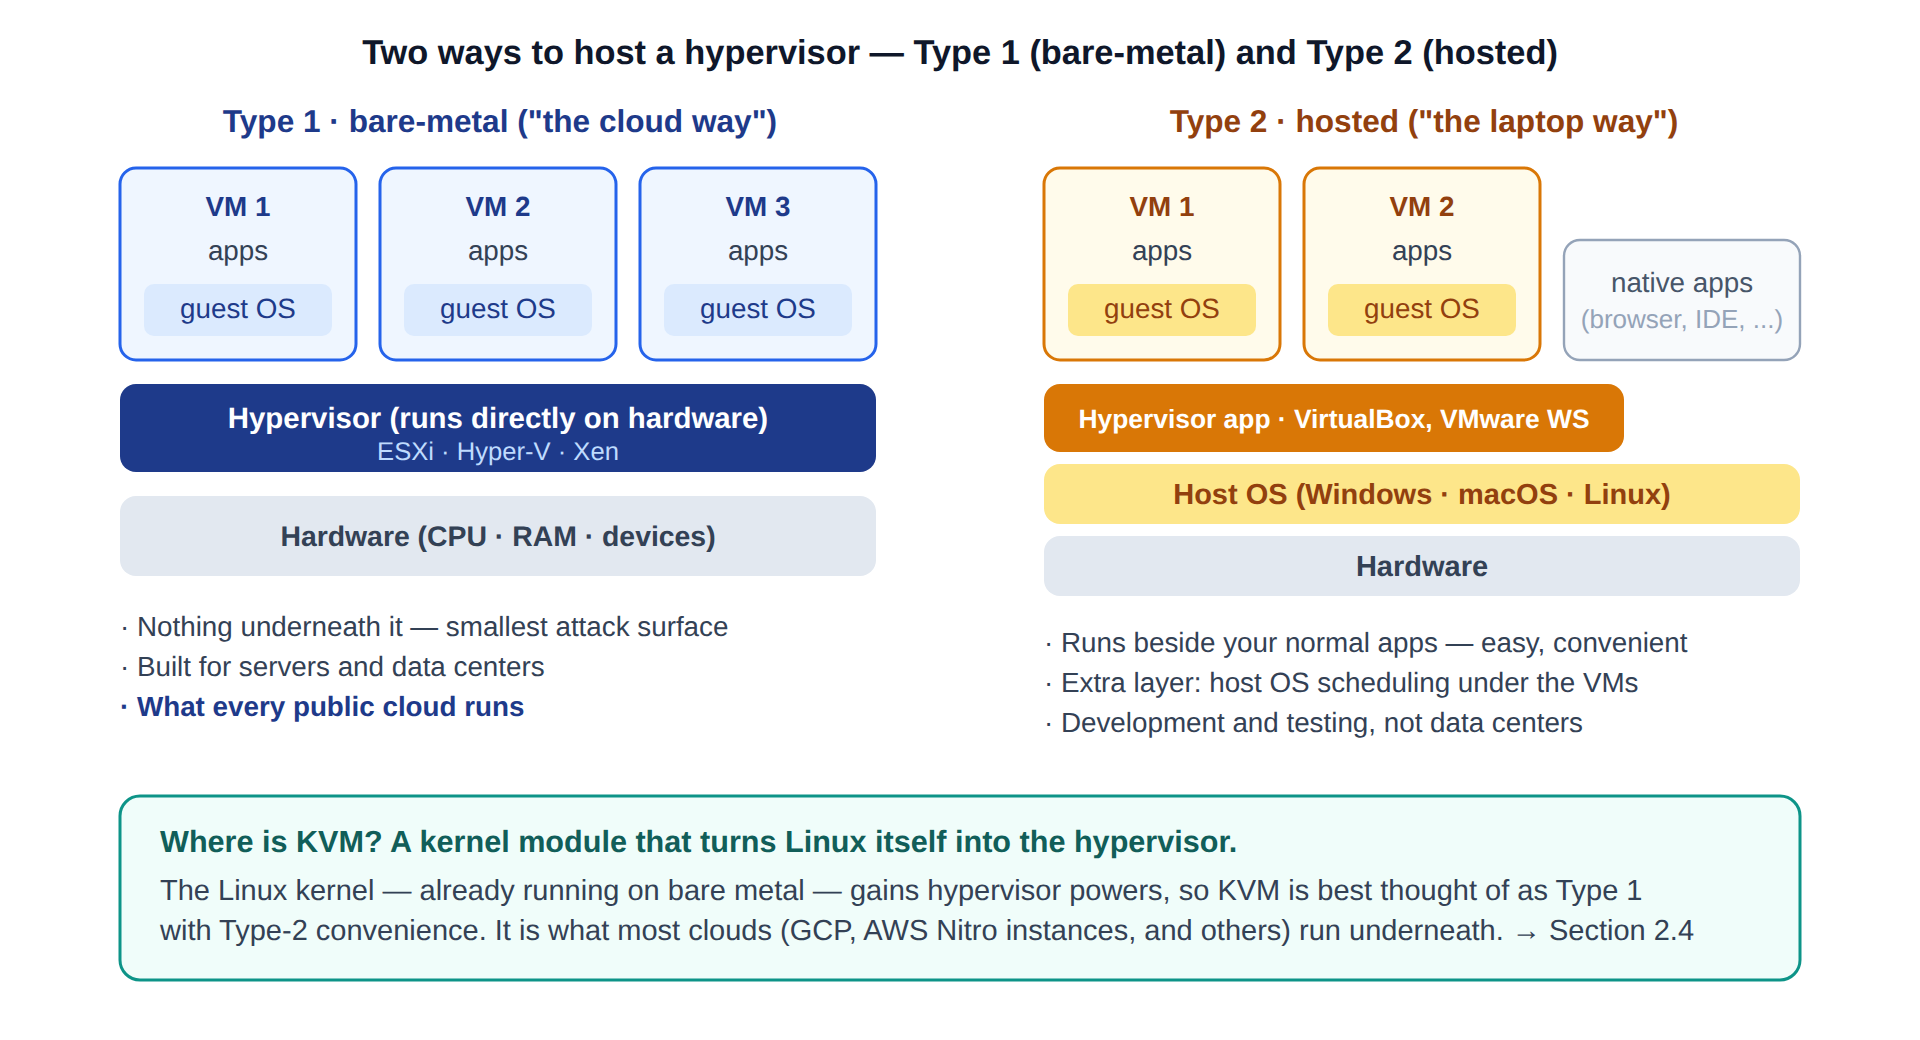
\includegraphics{figures/fig2-1_hypervisors.png}}\\[3pt]
  \figcaption{그림 2-1  Type 1(베어 메탈)과 Type 2(호스팅형) 하이퍼바이저. KVM은 경계를 흐린다. 이미 베어 메탈에서 실행되는 Linux 커널을 하이퍼바이저로 바꾸는 커널 모듈이다.}
\end{tbbfigure}

세계에서 가장 중요한 하이퍼바이저는 이 이분법을 거부한다. \textbf{KVM}은 Linux 커널 모듈이므로 "호스트 OS"와 "하이퍼바이저"가 같은 것이 된다. 이미 베어 메탈에서 실행 중인 Linux 자체가 VMM 능력을 얻는다. 실용적으로는 \textit{Type 2의 사용 편의성을 갖춘 Type 1}로 분류할 수 있다. 아키텍처는 하이퍼바이저급이지만, VM은 일반 Linux 도구로 일반 Linux 프로세스처럼 관리한다. 이 조합에 오픈 소스라는 장점까지 더해져 KVM은 Google Cloud, 현대 AWS (Nitro), OpenStack 클라우드, 그리고 이 장의 2.4절을 떠받친다.

\begin{calloutbox}{tbbpurple}{tbbpurplefill}
{\normalsize\bfseries\color{tbbpurple}생각해 보기}\par\vspace{3pt}
\begin{tbbitemize}
  \item Docker Desktop의 Linux VM을 실행하는 MacBook, GCP 호스트, WSL2를 실행하는 Windows를 분류해 보자. (힌트: WSL2는 Hyper-V에서 실행되며, Hyper-V는 실행 중인 Windows \textit{아래로} 들어간다.) 각각 어느 유형이며, 이 질문에 깔끔한 답이 있기는 한가?
  \item 바이너리 변환은 복잡성을 대가로 동등성을 보존했고, 반가상화는 속도를 위해 동등성을 희생했다. 오늘날에도 각 절충이 옳은 상황을 하나씩 제시해 보자.
\end{tbbitemize}
\end{calloutbox}

\section{하드웨어 지원 가상화: VT-x, VMCS, EPT}

2005\textasciitilde{}2006년, Intel과 AMD는 소프트웨어가 몸을 비틀며 피하려 했던 일을 했다. 프로세서를 바꿨다. Intel의 \textbf{VT-x}와 AMD의 \textbf{AMD-V}는 명령어 17개를 하나씩 고치는 대신 CPU에 완전히 새로운 특권 차원을 추가하여 x86이 마침내 Popek \& Goldberg의 조건을 충족하게 했다. 이론에 앞서 실제 머신에서 해결책을 찾아보자. \code{grep} 한 번이면 된다.

\begin{terminalbox}
\begin{Verbatim}[breaklines=true,breakanywhere=true,fontsize=\small,formatcom=\color{tbbtermfg},codes=\tbbcodeactive]
# on any modern laptop / workstation running Linux:
$ grep -m1 -c -E "vmx|svm" /proc/cpuinfo
1                          # vmx = Intel VT-x, svm = AMD-V. 2005's fix.
$ ls -l /dev/kvm
crw-rw---- 1 root kvm 10, 232 Jul  6 09:14 /dev/kvm
#   ^ the kernel offering hypervisor powers as a device file (sec. 2.4)

# now the same two commands on this week's rented EC2 guest:
$ grep -m1 -c -E "vmx|svm" /proc/cpuinfo
0                          # the flag is gone. and /dev/kvm does not exist.
# the hypervisor HID it: your guest may not host guests of its own.
# the illusion, by default, refuses to nest.
\end{Verbatim}
\end{terminalbox}
\figcaption{기록 2-1  VT-x 찾기. 물리 노트북은 vmx/svm을 알리고 /dev/kvm을 공개한다. 임대한 VM 안에서는 하이퍼바이저가 이 기능을 마스킹한다. 곧 만날 VMCS가 선택한 CPUID 비트 하나다.}

\subsection*{두 세계: VMX root 모드와 non-root 모드}

VT-x는 링과 \textit{직교하는} 모드 전환을 추가한다(그림 2-2). 하이퍼바이저는 실제 머신을 완전히 제어하며 자체 rings 0–3을 지닌 \textbf{VMX root 모드}에서 실행된다. 게스트는 하드웨어의 감독을 받으면서 \textit{역시} rings 0–3을 지닌 \textbf{VMX non-root 모드}에서 실행된다. 이 문장을 두 번 읽어 보자. 오래된 딜레마가 사라진다. \textbf{게스트 커널은 다시 ring 0에서}, 작성된 그대로 실행되므로 보기 흉한 링 압축 묘수가 필요 없다. non-root ring 0은 진짜 ring 0이 아닐 뿐이다. CPU 자체가 게스트 실행을 감시하며, 하이퍼바이저가 개입할 가치가 있다고 표시한 작업이 일어나면 하드웨어가 \textbf{VM exit}를 수행해 자동으로 세계 전체를 root 모드로 전환한다. 처리가 끝나면 하이퍼바이저가 \textbf{VM entry}를 실행하고 게스트는 아무것도 모른 채 재개한다. 마침내 \textit{하드웨어}가 트래핑하는 트랩 후 에뮬레이션이 완성되고, 문제의 명령어 17개도 다른 것처럼 트랩한다.

\begin{tbbfigure}
  \adjustbox{max width=0.94\linewidth,max totalheight=0.46\textheight}{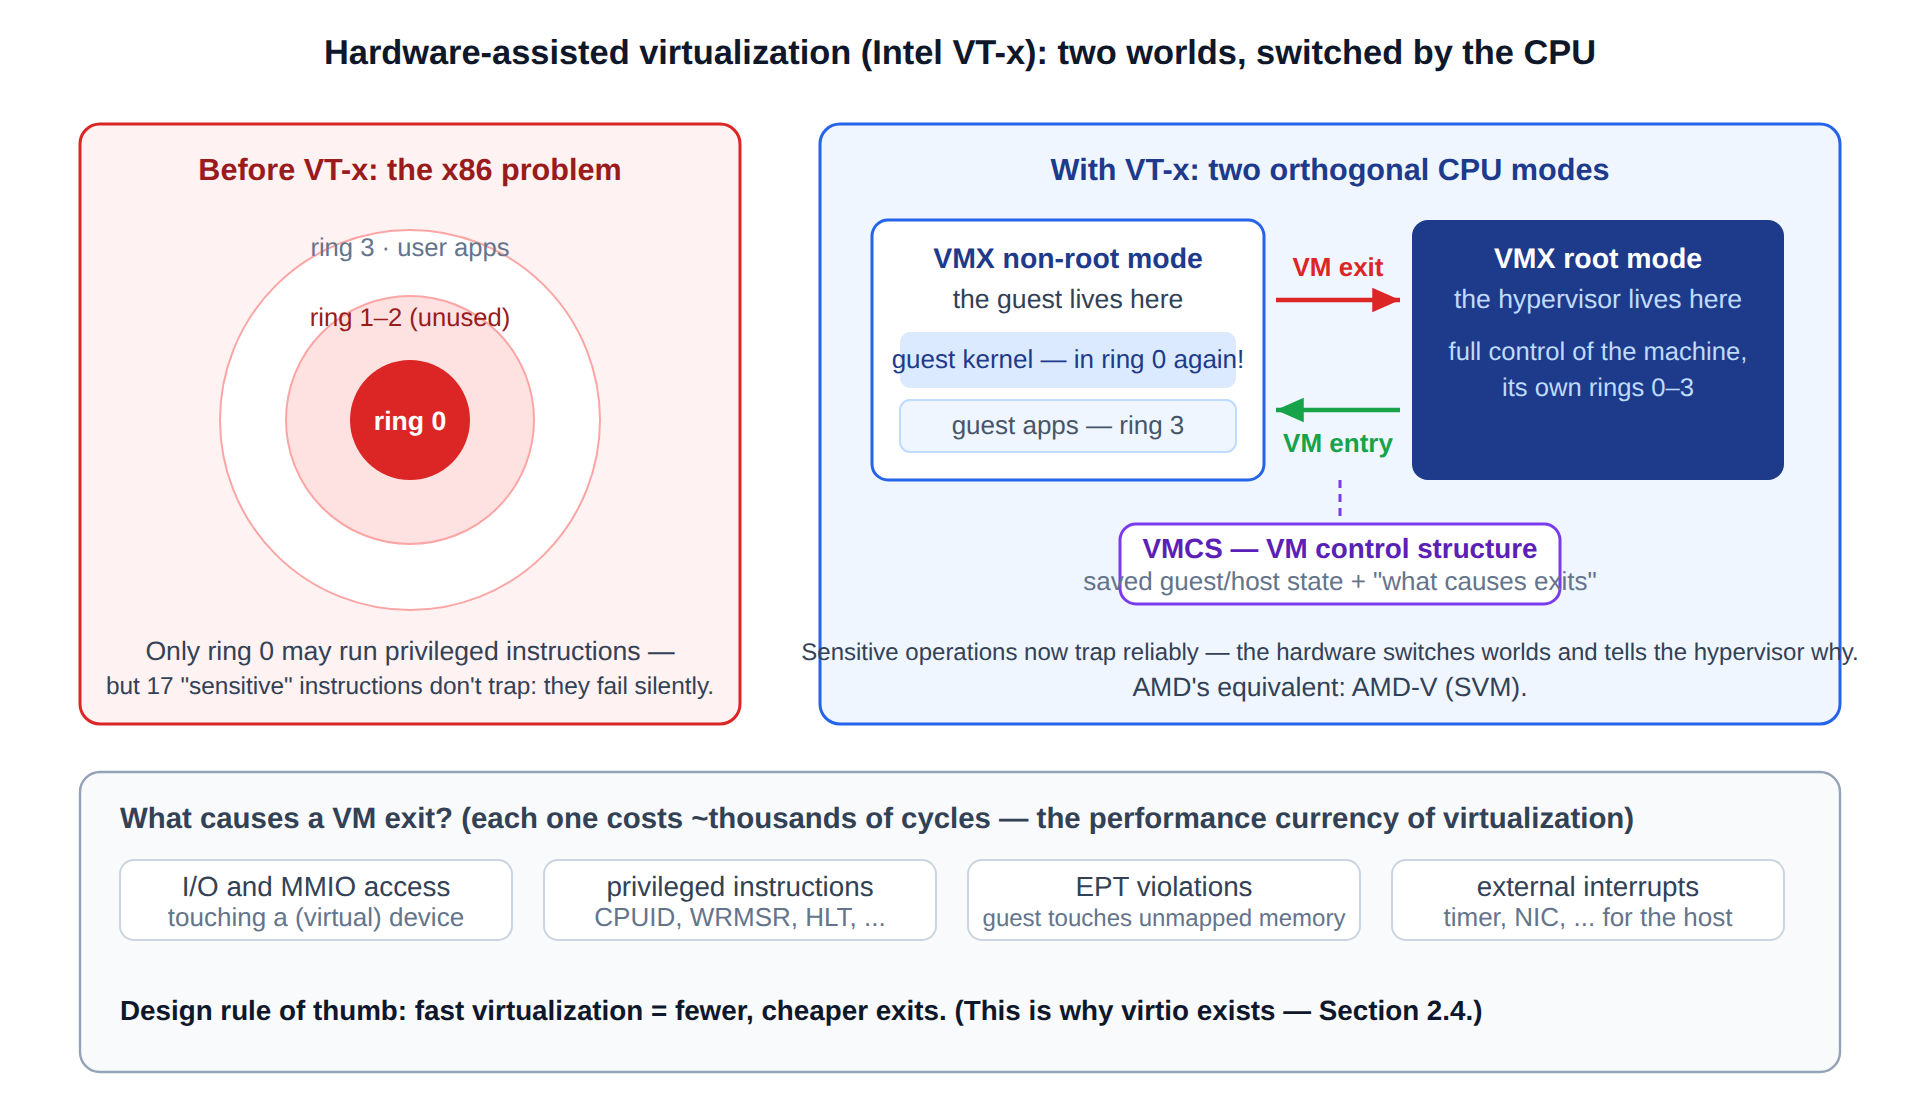
\includegraphics{figures/fig2-2_vtx.png}}\\[3pt]
  \figcaption{그림 2-2  한 장으로 보는 VT-x. 왼쪽은 2005년 이전의 문제로, 특권이 낮아진 게스트 커널과 조용히 실패하는 명령어를 보여 준다. 오른쪽은 root/non-root 모드, VM exit와 entry, 규칙과 상태를 기록하는 VMCS다.}
\end{tbbfigure}

\subsection*{VMCS: 두 세계 사이의 계약}

세계를 전환할 때는 두 세계의 상태와 교전 규칙을 보관할 곳이 필요하다. 그것이 가상 CPU마다 하나씩 존재하는 \textbf{VMCS (Virtual Machine Control Structure)}다. (a) entry 때 로드하고 exit 때 저장하는 게스트 레지스터 상태, (b) exit 때 복원하는 호스트 상태, (c) 하이퍼바이저가 하드웨어를 프로그래밍하는 \textbf{제어 필드}를 담는다. 어떤 이벤트가 exit를 일으키는지(\code{CPUID}가 exit해야 하는가? 모든 I/O 포트 접근은? 이 제어 레지스터에 쓰기는?), 특정 기능을 게스트에 어떻게 보일지, exit 핸들러가 어디에 있는지를 정한다. exit가 발생하면 하드웨어는 \textbf{exit 이유}도 VMCS에 기록한다. 따라서 하이퍼바이저의 핵심은 문자 그대로 exit 이유를 처리하는 거대한 \code{switch} 문이다. 2.4절에서 KVM 실행 루프를 볼 때 바로 이 구조를 구동한다.

\subsection*{Exit는 가상화 성능의 통화다}

VM exit는 아키텍처상 무거운 작업이다. 한 세계를 저장하고 다른 세계를 로드한다. 캐시 효과까지 세면 왕복에 대략 마이크로초가 걸리며, 최선의 경우에도 CPU 수천 사이클이 든다. exit가 드문 게스트는 사실상 네이티브 속도로 실행되지만, 계속 exit하는 게스트는 기어간다. 이 한 문장이 20년의 가상화 엔지니어링을 정리한다.

\begin{tbbitemize}
  \item \textbf{Exit 횟수를 줄인다.} 과거 하이퍼바이저가 처리하던 작업을 하드웨어가 non-root 모드에서 처리하게 한다(아래의 EPT, 인터럽트용 APICv). 레지스터 쓰기마다 exit하지 않고 exit 한 번에 작업을 배치하는 장치 인터페이스를 설계한다(virtio, 2.4절).
  \item \textbf{남은 exit를 저렴하게 만든다.} CPU 세대가 거듭되면서 세계 전환 지연 시간이 줄었다. 하이퍼바이저는 빈번한 exit를 가벼운 커널 경로로 보내고 드물고 복잡한 것만 사용자 공간에 맡긴다.
\end{tbbitemize}

실습 이후에도 이 관점을 유지하자. 가상화된 워크로드의 성능이 수수께끼처럼 낮으면 실무자가 가장 먼저 묻는 질문은 \textit{무엇이 얼마나 자주 exit하는가}다. 호스트의 \code{perf kvm stat} 같은 도구는 exit를 이유별로 표로 만들어 정확히 답한다. VM의 "exit 폭풍"은 프로세스의 시스템 호출 폭풍과 같다.

\subsection*{두 번째 문제: 섀도 페이지에서 EPT까지}

CPU 가상화는 전투의 절반에 불과했다. 나머지 절반은 메모리다. 이제 주소 변환에 \textbf{두 겹의 거짓말}이 있기 때문이다(그림 2-3). 게스트 OS는 게스트 가상 주소를 \textbf{게스트 물리} 주소로 변환하는 페이지 테이블을 만든다. 그러나 게스트 물리 주소 자체도 허구이며, 게스트 페이지가 \textbf{호스트 물리} 메모리의 어디에 실제로 위치하는지는 하이퍼바이저가 정한다. 2008년 이전의 하드웨어 페이지 테이블 워커는 테이블 집합 하나만 따라갈 수 있었다. 두 변환을 합칠 무언가가 필요했다.

\begin{tbbfigure}
  \adjustbox{max width=0.94\linewidth,max totalheight=0.46\textheight}{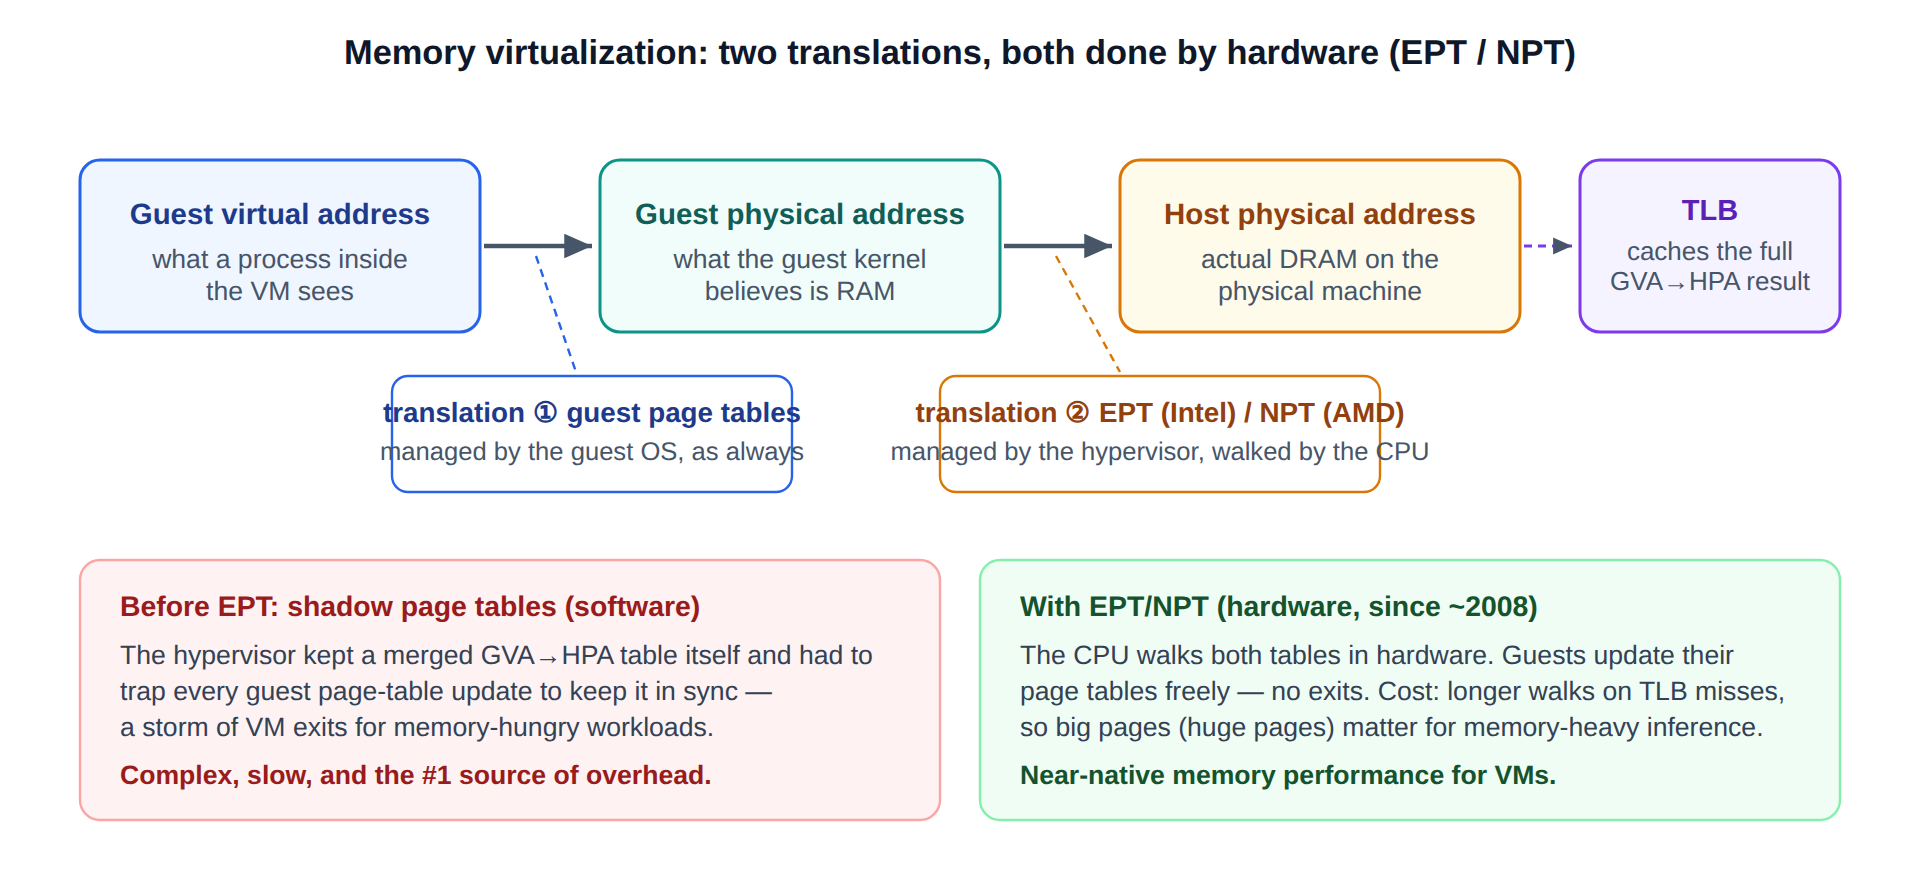
\includegraphics{figures/fig2-3_ept.png}}\\[3pt]
  \figcaption{그림 2-3  메모리 가상화. 게스트 페이지 테이블(게스트 관리)과 EPT/NPT(하이퍼바이저 관리)의 두 변환을 모두 하드웨어가 순회하며, TLB가 합성된 결과를 캐시한다.}
\end{tbbfigure}

소프트웨어 시대의 답은 \textbf{섀도 페이지 테이블}이었다. 하이퍼바이저가 게스트 주소 공간마다 게스트 가상→호스트 물리 변환을 합친 테이블을 유지하고 실제 하드웨어가 이를 순회했다. 게스트 페이지 테이블을 쓰기 보호하고 \textbf{모든 게스트 페이지 테이블 갱신을 트랩}하여 일관성을 유지했다. 프로세스를 포크하거나 메모리의 넓은 영역에 접근하는 워크로드에서는 exit 폭풍과 고통스러운 성능 저하가 발생했다. 섀도 페이징은 가상화 오버헤드와 복잡성의 가장 큰 단일 원인이었다.

하드웨어의 답은 Intel의 \textbf{EPT}(Extended Page Tables, \textasciitilde{}2008)와 AMD의 \textbf{NPT}로 등장했다. CPU가 게스트 자체의 페이지 테이블에 \textit{더해} 순회하는, 하이퍼바이저 소유의 \textit{두 번째} 페이지 테이블 집합이다. 게스트는 트랩, 섀도, exit 없이 자유롭게 테이블을 갱신한다. 대가는 정직하고 눈에 보인다. 이제 TLB 미스에는 2차원 순회가 필요하다. 최악에는 게스트의 4–5개 레벨마다 자체 EPT 순회가 필요해 최대 \textasciitilde{}24번의 메모리 참조가 일어난다. 따라서 \textbf{VM에서는 TLB 미스가 더 아프다.} 일반적인 완화책은 4 KB 대신 2 MB / 1 GB인 \textbf{대형 페이지}를 사용해 TLB 압력을 크게 줄이는 것이다. 추론 서버는 수 기가바이트 가중치 텐서를 보관하는 메모리 집약적 워크로드라 이 차이를 알아차리므로 이 과정에서도 기억할 가치가 있다. EPT와 exit가 줄어든 인터럽트 처리를 함께 사용하면 잘 구성한 VM의 계산 및 메모리 성능은 베어 메탈과 몇 퍼센트 이내 차이에 그친다. 클라우드를 그 위에 세울 수 있는 이유다.

CPU와 메모리는 해결했다. 세 번째 기둥인 \textbf{I/O}에서 아키텍처 이야기가 특히 흥미로워진다. Linux, QEMU, virtio라는 반가상 아이디어가 등장하기 때문이다. 다음 절의 주제다.

\begin{calloutbox}{tbbpurple}{tbbpurplefill}
{\normalsize\bfseries\color{tbbpurple}생각해 보기}\par\vspace{3pt}
\begin{tbbitemize}
  \item 다음 게스트 작업을 "계속 exit함"부터 "전혀 exit하지 않음"까지 순서대로 놓고 근거를 설명해 보자. 두 레지스터 더하기, 에뮬레이션 직렬 포트에서 한 바이트 읽기, TLB 히트인 메모리 로드, CPUID 실행, 자체 페이지 테이블 갱신(EPT 시대).
  \item EPT는 게스트 페이지 테이블 갱신에서 exit를 없앴지만 TLB 미스의 비용을 높였다. 30 GB LLM 가중치 버퍼를 4 KB 페이지와 1 GB 대형 페이지로 접근할 때 각각 대략 몇 개의 TLB 엔트리가 필요한가? 무엇을 시사하는가?
\end{tbbitemize}
\end{calloutbox}

\section{KVM, QEMU, virtio: 클라우드의 하이퍼바이저가 된 Linux}

VT-x는 모든 운영체제에 하이퍼바이저의 원재료를 제공했다. Linux는 거의 즉시 이를 차지했다. \textbf{KVM (Kernel-based Virtual Machine)}은 2007년 초 메인라인 커널에 병합되었으며, 재사용 설계의 작은 걸작이다. 하이퍼바이저 역할을 위해 스케줄러, 메모리 관리자, 드라이버를 모두 갖춘 새 운영체제를 만드는 대신, KVM은 Linux에 이미 세 기능의 세계적 구현이 \textit{모두} 있다는 점에 주목하고 VT-x를 구동하는 법만 가르쳤다. 그 결과가 앞으로 사용할 클라우드 대부분의 아래에 있는 소프트웨어 스택이며, 작업을 세 부분으로 나눈다(그림 2-4).

\begin{tbbfigure}
  \adjustbox{max width=0.94\linewidth,max totalheight=0.46\textheight}{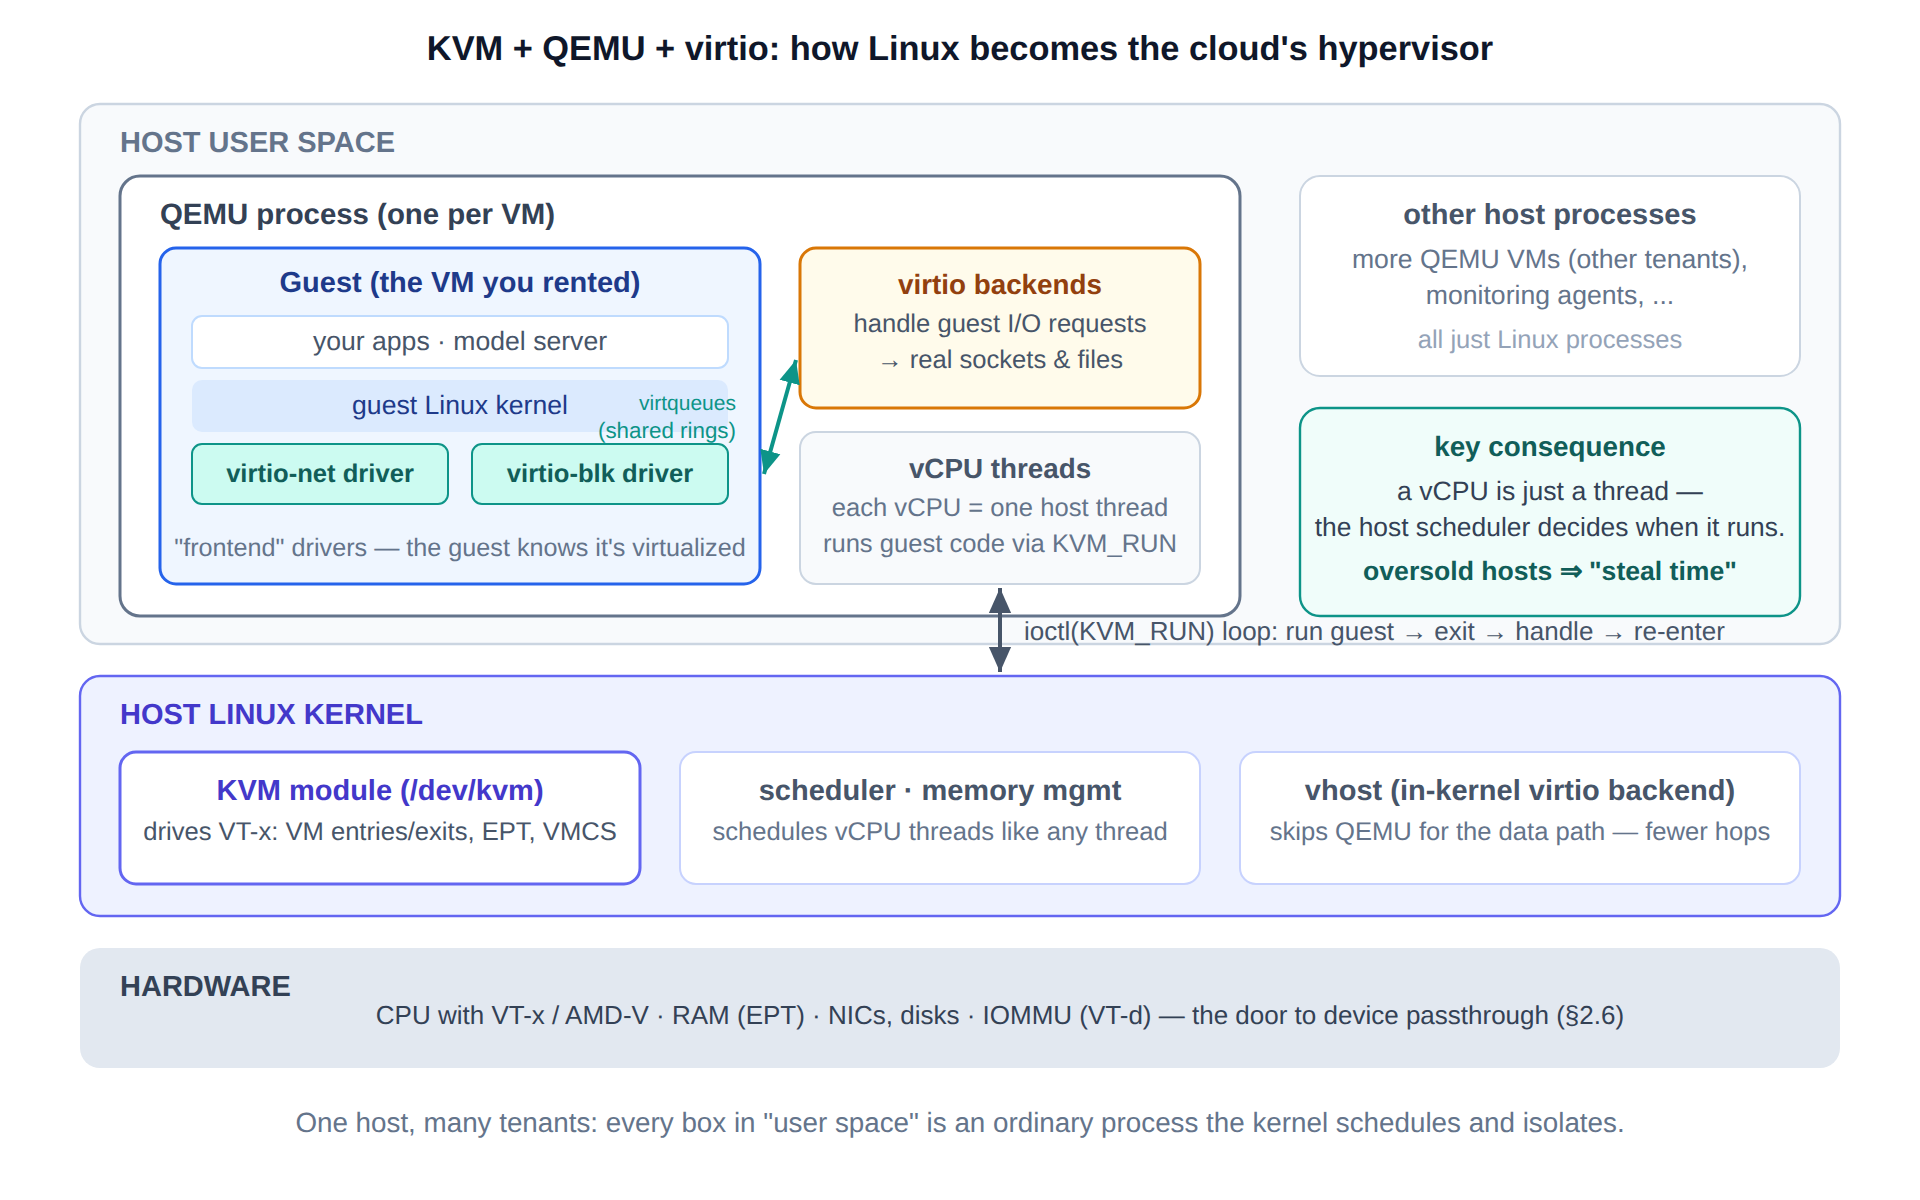
\includegraphics{figures/fig2-4_kvm_virtio.png}}\\[3pt]
  \figcaption{그림 2-4  KVM/QEMU/virtio 스택. KVM(커널)은 VT-x를 구동하고, QEMU(VM당 사용자 공간 프로세스 하나)는 장치를 제공하며, virtio는 하드웨어의 환상을 정직하고 빠른 인터페이스로 바꾼다. vCPU는 그저 호스트 스레드다.}
\end{tbbfigure}

\subsection*{작업 분담}

\begin{tbbitemize}
  \item \textbf{KVM(커널 안)}은 작은 ioctl API인 \code{/\allowbreak dev/\allowbreak kvm}을 공개한다. VM 생성, 메모리 제공, vCPU 생성, 그리고 핵심인 \code{KVM\_RUN}이다. VMCS를 프로그래밍하고 VM entry를 실행하며 VM exit를 받아 처리한다. 빈번하고 단순한 exit(EPT 폴트, 대부분의 MSR 접근)는 커널에서 바로 처리한다.
  \item \textbf{QEMU(사용자 공간, VM당 프로세스 하나)}는 나머지 모든 일을 한다. 게스트 메모리(그저 프로세스 메모리다!)를 할당하고, 펌웨어나 커널을 로드하며, 대표적인 역할인 \textbf{장치 모델}을 제공한다. NIC, 디스크, 직렬 포트와 마더보드의 나머지 장치를 소프트웨어로 가장한다. 장치 I/O 때문에 VM exit가 발생하면 KVM이 QEMU로 넘긴다. QEMU 장치 코드는 게스트가 "하드웨어"에 무슨 일을 하려 했는지 파악하고 일반 Linux 시스템 호출을 통해 현실의 동등한 작업을 한다. 실제 소켓에 패킷을 보내거나 실제 파일에 블록을 쓴다.
  \item \textbf{호스트 Linux 커널}은 둘 다 다시 구현하지 않는 기능을 제공한다. 스케줄러가 vCPU를 실행하고, 메모리 관리자가 게스트 RAM을 뒷받침하며, 드라이버와 파일 시스템이 실제 I/O를 운반한다.
\end{tbbitemize}

게스트를 움직이는 실행 루프를 한 번은 문장으로 살펴볼 가치가 있다. vCPU 스레드가 \code{ioctl(KVM\_RUN)}을 호출하고, 커널이 VM entry를 수행한다. 게스트는 무언가 exit할 때까지 non-root 모드에서 네이티브로 계산한다. KVM은 exit를 처리하고 즉시 다시 entry하거나, 장치 작업을 위해 QEMU로 돌아갔다가 다시 entry한다. VM의 수명 내내 이 과정이 반복된다. 2.3절에서 배운 exit 이유와 exit 비용은 모두 이 루프 내부의 경제성이다.

\subsection*{vCPU는 그저 스레드다 — p99가 신경 써야 하는 이유}

그림 2-4에서 vCPU가 어디에 있는지 다시 보자. \textbf{일반 호스트 스레드}다. 그림의 말만 믿지 않아도 된다. KVM 게스트를 실행하는 Linux 머신이라면 어느 것이든 호스트가 직접 보여 준다(virt-manager를 사용하는 노트북이면 충분하다).

\begin{terminalbox}
\begin{Verbatim}[breaklines=true,breakanywhere=true,fontsize=\small,formatcom=\color{tbbtermfg},codes=\tbbcodeactive]
# on the HOST, with one 4-vCPU guest running:
$ pstree -p $(pgrep -of qemu) | head -5
qemu-system-x86(9114)-+-{CPU 0/KVM}(9131)
                      |-{CPU 1/KVM}(9132)
                      |-{CPU 2/KVM}(9133)
                      |-{CPU 3/KVM}(9134)
$ ps -o pid,psr,pcpu,comm -Lp 9114 | grep CPU  # psr = core hosting it
 9131  3  99.2  CPU 0/KVM     # "processor 0" = thread 9131, on core 3
 9132 11   1.0  CPU 1/KVM     # idle vCPU, parked on core 11
# renice it, pin it, cgroup it - everything Linux does to threads applies.
\end{Verbatim}
\end{terminalbox}
\figcaption{기록 2-2  호스트에서 본 게스트의 "프로세서" 네 개. QEMU 프로세스 하나 안에 있는 스케줄 가능한 스레드 네 개다. 이후의 오버커밋, 스틸 타임, 전용 코어는 모두 평범한 스레드 스케줄링이 의상을 입은 것이다.}

이 한 가지 사실에서 운영 중 만나게 될 여러 클라우드 현상이 나온다.

\begin{tbbitemize}
  \item \textbf{오버커밋.} 호스트는 테넌트의 최대 부하가 동시에 오지 않을 것에 베팅하며 물리 코어보다 많은 vCPU를 만들 수 있다. 항공 좌석과 같은 경제성이다. 저가 인스턴스 계열은 이 베팅을 바탕으로 가격이 정해진다.
  \item \textbf{스틸 타임.} vCPU가 실행 가능할 때 호스트 스케줄러가 \textit{다른 누군가}를 실행하면 게스트는 사이클을 얻지 못한 채 시간이 흐르는 경험을 한다. 게스트 안의 \code{top}에서는 \code{\%st}로 보인다. 지연 시간에 민감한 서빙에서 스틸 타임은 순수한 꼬리 지연 시간 독극물이다. 빼앗긴 슬라이스에 도착한 요청은 보이지 않게 기다린다. 진지한 서빙 서버군이 전용 코어 인스턴스 유형을 구매하는 이유이며, "CPU 그래프는 멀쩡한데 p99가 급증한다"는 질문의 답이 VM 한 계층 아래에 있을 수 있는 이유다.
  \item \textbf{시끄러운 이웃, 그러나 경계가 있다.} 스케줄러와 cgroup 가중치(제3장!)는 테넌트가 서로 해칠 수 있는 정도를 제한한다. 2.1절의 심판은 다음 주에 직접 다룰 바로 그 커널 메커니즘으로 구현된다.
\end{tbbitemize}

스틸 타임은 별도 사례로 살펴볼 가치가 있다. 프로덕션 텔레메트리에서 만날 가능성이 가장 높은 가상화 산물이며, 애플리케이션 문제로 오진하기도 가장 쉽다.

\begin{terminalbox}
\begin{Verbatim}[breaklines=true,breakanywhere=true,fontsize=\small,formatcom=\color{tbbtermfg},codes=\tbbcodeactive]
# inside a guest on a busy (oversold) host, during a load test:
$ top -bn1 | grep "%Cpu"
%Cpu(s): 41.2 us, 3.1 sy, 0.0 ni, 30.5 id, 0.2 wa, 0.0 hi, 0.6 si, 24.4 st
#                                                                  ^^^^^^^
# st = steal: 24.4% of this guest's runnable time went to... someone else.
# no process inside the guest will ever show this in its profile.
$ grep -A1 steal /proc/stat | head -2      # the raw counter, if you script it
cpu  184023 340 44522 830112 902 0 4211 267001 0 0
#                                        ^^^^^^ jiffies stolen since boot
\end{Verbatim}
\end{terminalbox}
\figcaption{기록 2-3  현장에서 붙잡은 스틸 타임. 게스트는 실행 가능했지만 호스트 스케줄러가 다른 테넌트를 실행했고, 요청은 볼 수 없는 슬라이스를 기다렸다. 깨끗한 CPU 그래프와 함께 p99가 급증한다면 한 계층 아래에 답이 있다.}

\subsection*{장치 문제와 virtio의 정직한 답}

이제 가상화의 세 번째 기둥인 I/O를 살펴보자. 완전한 환상을 제공하는 방식은 \textbf{장치 에뮬레이션}이다. QEMU가 오래되고 유명한 특정 실제 NIC를 가장하고(고전적인 예는 Intel e1000), 게스트는 기본 드라이버를 실행한다. e1000 드라이버가 있는 모든 OS가 바로 작동하므로 동등성은 완벽하다. 그러나 대가를 생각해 보자. 이 드라이버는 레지스터 쓰기가 나노초밖에 걸리지 않는 하드웨어용으로 작성되었다. 에뮬레이션 장치에서는 \textbf{모든 레지스터 접근이 사용자 공간으로 향하는 VM exit}다. 패킷 하나를 보내면서 장치를 여러 번 건드린다. exit, exit, exit다. 에뮬레이션 I/O는 세계 전환에 빠져 네이티브보다 10배 이상 느릴 수 있다.

해결책은 2.2절의 반가상 아이디어를 가장 잘 맞는 곳에서 되살리는 것이다. \textbf{virtio}(Rusty Russell, 2008, 현재 표준)는 가장을 멈추라고 말한다. 게스트에 \textit{공공연히 가상인} 장치를 제공하되, 소프트웨어 구성 요소 두 개가 공유 메모리로 버퍼를 전달하는 실제 상황에 맞게 인터페이스를 설계한다. 게스트는 \textbf{프런트엔드 드라이버}(\code{virtio-net}, \code{virtio-blk}, ...)를 로드하고, 하이퍼바이저 쪽은 짝이 되는 \textbf{백엔드}를 실행한다. 둘 사이에는 \textbf{virtqueue}가 있다. 게스트가 버퍼 디스크립터를 배치로 올리고 백엔드가 소비하는 게스트 메모리의 링 버퍼다. 게스트는 레지스터마다가 아니라 \textit{배치마다} 가벼운 exit 한 번으로 백엔드를 "깨운다". 완료 신호는 인터럽트로 돌아오거나 폴링 중에 수거한다. 부하가 걸리면 링이 계속 바쁘게 돌아가므로 exit가 거의 없다. 한 계층 아래에서 10주 차 동적 배칭과 같은 물리 법칙이 작동한다. \textbf{비싼 경계 통과 비용을 여러 작업 단위에 분산한다.}

두 가지 개선으로 그림이 완성된다. \textbf{vhost}는 백엔드를 QEMU에서 호스트 커널로 옮겨 데이터 경로의 사용자 공간 홉을 없앤다(vhost-user는 DPDK 기반 네트워크 스택처럼 전용 사용자 공간 스위치로 옮긴다). 최고 등급에서는 하드웨어가 다시 등장한다. \textbf{SR-IOV}는 물리 NIC 하나가 가벼운 \textit{가상 함수} 여러 개를 제공하게 하며, 각 함수를 IOMMU를 통해 게스트에 곧바로 안전하게 할당할 수 있다. 실리콘 자체가 장치 "에뮬레이션"을 하는 셈이다. 이 생각을 붙들어 두자. 실제 하드웨어를 게스트에 할당하는 방식은 2.6절에서 GPU가 VM에 도달하는 방법과 정확히 같다.

\begin{calloutbox}{tbbteal}{tbbtealfill}
{\normalsize\bfseries\color{tbbx115E59}상자 2-2  AWS Nitro: 가상화 비용을 0에 가깝게}\par\vspace{3pt}
이 절의 논리를 끝까지 따라가면 현대 EC2 아래의 시스템인 Nitro에 도달한다. AWS는 장치 모델을 \textit{소프트웨어 밖으로 완전히} 옮겼다. 네트워킹, 스토리지, 관리는 전용 \textbf{Nitro 카드}(맞춤형 실리콘)에서 실행되고 게스트에는 직접 할당된 하드웨어로 제공된다. 호스트 CPU에는 의도적으로 최소화한 KVM 기반 하이퍼바이저만 남으며 데이터 경로에 QEMU가 없다. 게스트는 베어 메탈에 가까운 성능을 얻고, 호스트는 배관에 코어를 거의 쓰지 않는다. 같은 아키텍처가 진정한 베어 메탈 인스턴스도 제공한다(Nitro 카드가 마더보드의 I/O \textit{자체}다). 역사의 흐름은 깔끔하다. EC2는 반가상화된 Xen에서 시작했고(2006), 20년에 걸친 exit 제거는 exit가 하던 일을 하드웨어로 옮기며 끝났다(2017–).
\end{calloutbox}

\vspace{3.0pt}

\begin{calloutbox}{tbbpurple}{tbbpurplefill}
{\normalsize\bfseries\color{tbbpurple}생각해 보기}\par\vspace{3pt}
\begin{tbbitemize}
  \item 게스트의 모델 서버에서 클라이언트로 나가는 HTTPS 응답 하나를 추적해 보자. (a) 에뮬레이션 e1000, (b) virtio + vhost, (c) SR-IOV에서 각 바이트가 그림 2-4의 어느 구성 요소를 통과하는가? 세계 전환 횟수를 정성적으로 세어 보자.
  \item 부하 테스트 중 지연 시간이 급증할 때 게스트 안의 \code{top}에 25\% steal이 나타난다. 클라우드 공급자를 바꾸지 않고 선택할 수 있는 방법은 무엇인가? (인스턴스 계열과 "전용"의 비용을 생각해 보자.)
\end{tbbitemize}
\end{calloutbox}

\section{VM은 얼마나 작아질 수 있는가? microVM과 격리 스펙트럼}

지금까지는 몇 시간에서 몇 년 동안 사는 임대 서버라는 고전적인 클라우드 단위를 가정했다. 2010년대에는 새로운 극단이 등장했다. \textbf{밀리초에서 몇 분} 동안 살고, \textbf{서로 신뢰하지 않는 낯선 사용자}에게 속하며, 경제성을 확보하려면 \textbf{호스트 한 대에 수천 개}를 넣어야 하는 서버리스 함수와 요청별 샌드박스다. 환경 생성에 40 s와 500 MB가 든다면 100 ms 단위로 과금할 수 없으므로, 이 규모에서는 고전적 VM의 형태가 맞지 않는다. 산업의 대응은 가상화 자체를 바꾸었다. 이를 이해하려면 \textit{테넌트 코드와 호스트 커널 사이에 무엇이 있으며 각 계층의 비용은 얼마인가?}라는 스펙트럼으로 보아야 한다(그림 2-5).

\begin{tbbfigure}
  \adjustbox{max width=0.94\linewidth,max totalheight=0.46\textheight}{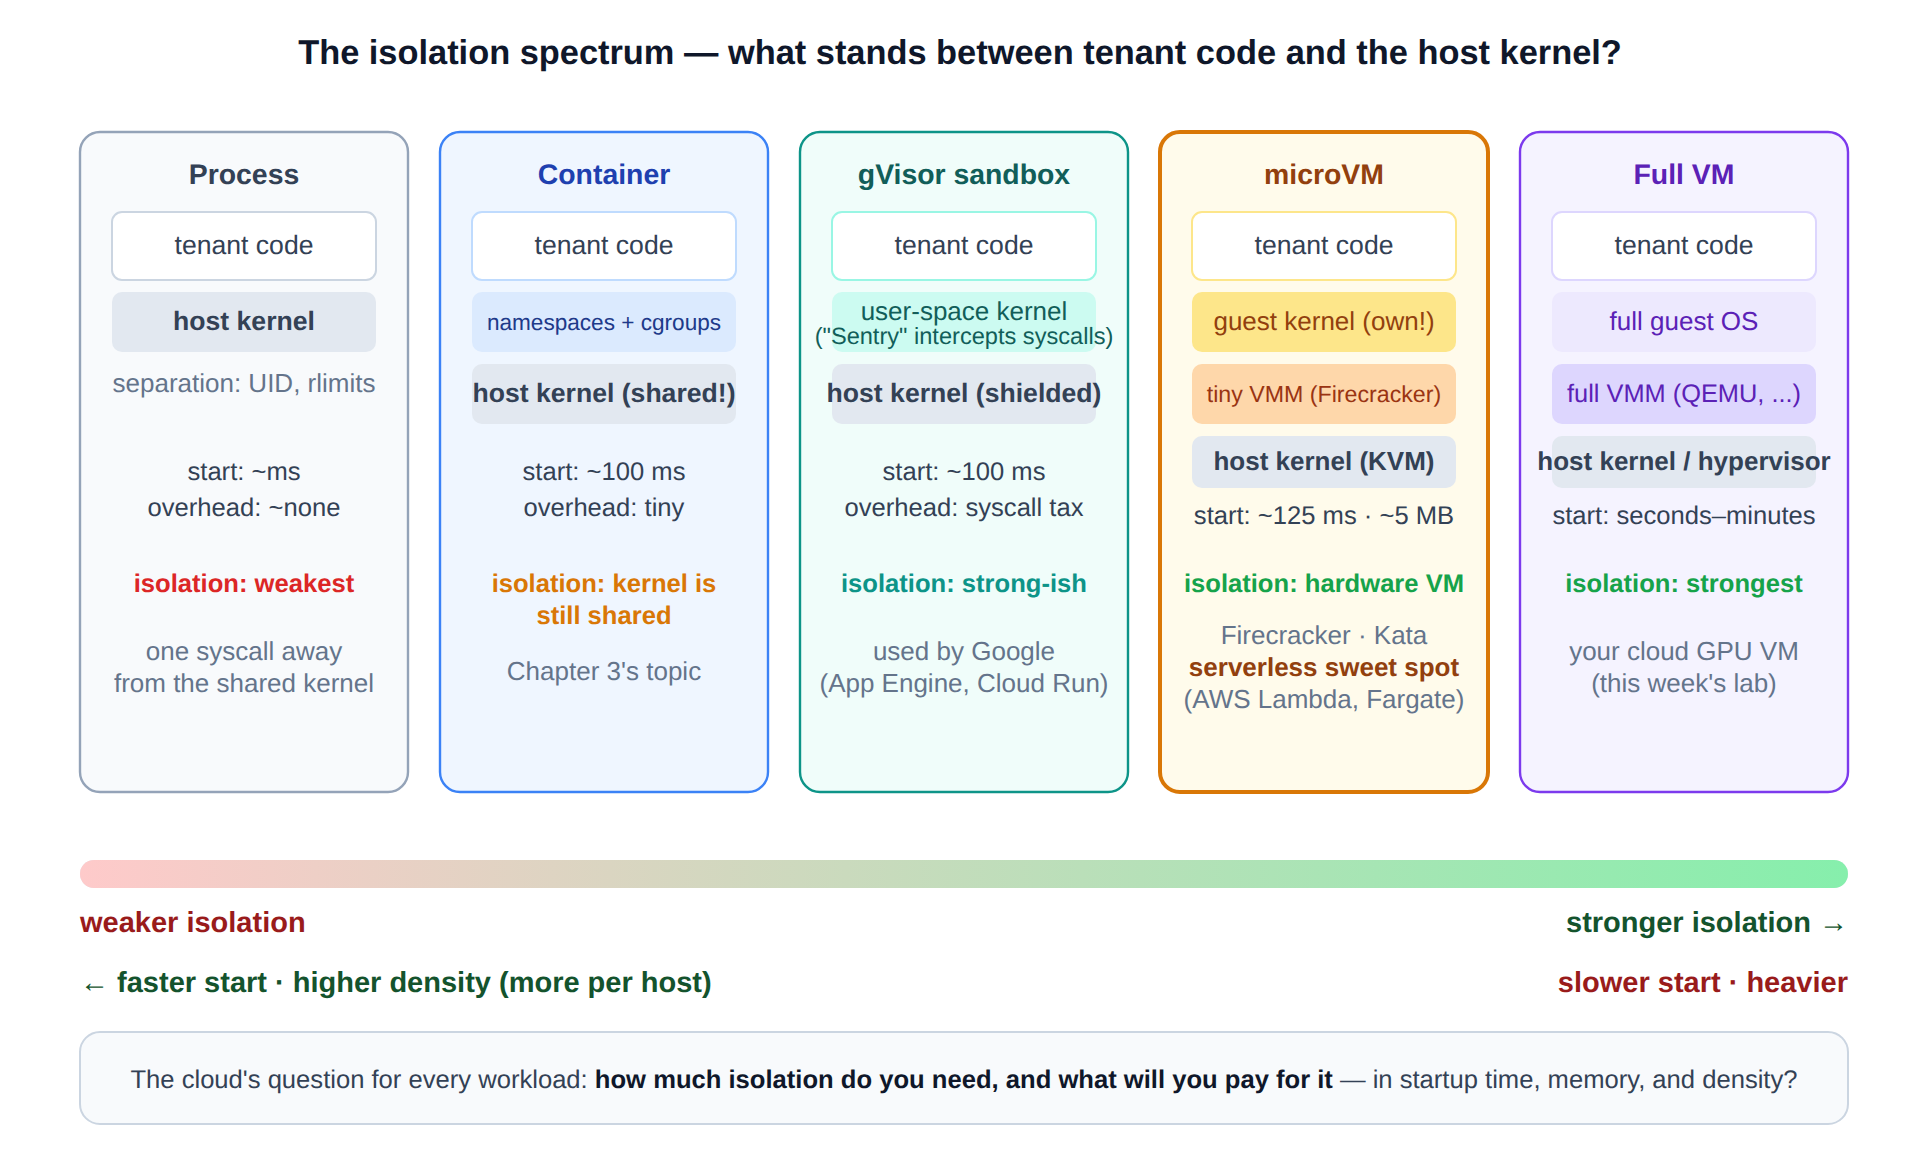
\includegraphics{figures/fig2-5_spectrum.png}}\\[3pt]
  \figcaption{그림 2-5  격리 스펙트럼. 오른쪽으로 갈수록 테넌트와 호스트 커널 사이의 계층이 많아지고 격리는 강해지지만 시작은 느려지고 밀도는 낮아진다. 서버리스의 최적 지점은 microVM이다.}
\end{tbbfigure}

\subsection*{컨테이너만으로 해결되지 않는 이유}

다음 주에는 커널 기본 요소로 컨테이너를 만들 것이므로 여기서는 보안에 관련된 윤곽만 보면 된다. 컨테이너는 일반 프로세스 묶음에 비공개 \textit{뷰}(네임스페이스)와 제한된 \textit{몫}(cgroup)을 제공한다. 그러나 \textbf{호스트의 다른 모든 사용자와 여전히 같은 커널을 공유한다.} 시작에는 \textasciitilde{}100 ms가 걸리고 오버헤드는 거의 0이므로 컨테이너가 패키징 전쟁에서 승리했다. 하지만 격리 경계는 시스템 호출 인터페이스다. 수백 개 진입점이 하나의 커널로 이어지며, 커널 취약점 하나가 모든 테넌트의 취약점이 된다. 컨테이너 탈출은 가설이 아니라 반복해서 등장하는 CVE 유형이다. \textit{자신의} 클러스터에서 \textit{자신의} 워크로드를 공유할 때는 보통 이 위험을 받아들일 수 있으며, Kubernetes도 바로 그 판단 위에 세워졌다. 그러나 공개 FaaS, CI 서비스, 모델이 생성한 프로그램을 실행하는 AI 에이전트 샌드박스처럼 \textbf{임의의 낯선 코드}를 실행할 때는 대부분 운영자가 공유 커널로 부족하다고 판단한다. (마지막 예시는 이 과정의 시대에 특히 중요하다. "LLM이 방금 작성한 코드를 실행한다"는 것은 멀티테넌트 격리 문제의 전형이다.)

\subsection*{컨테이너와 VM 사이의 세 가지 답}

\textbf{gVisor (Google, 2018)}는 컨테이너 형태를 유지하되 경호원을 넣는다. Go로 작성한 사용자 공간 커널인 \textit{Sentry}가 애플리케이션의 시스템 호출을 가로채 직접 처리하며, 대폭 줄이고 강화한 호출 집합으로 실제 호스트 커널에 접근한다. 따라서 테넌트 코드는 호스트 커널과 직접 통신하지 않는다. 커널 익스플로잇은 먼저 메모리 안전성을 갖춘 두 번째 커널을 뚫어야 한다. 대가는 시스템 호출 비용(I/O가 많은 워크로드가 체감한다)과 Linux 동작의 경계에서 발생하는 불완전한 호환성이다. Google은 App Engine, Cloud Run, Cloud Functions의 대규모 서버군에서 이를 사용한다.

\textbf{Kata Containers}는 반대 방향으로 간다. 컨테이너 \textit{인터페이스}는 유지하지만 \textit{구현}을 실제 하드웨어 VM으로 바꾼다. 각 pod는 경량 VM 안에 자체 게스트 커널을 가지며, 표준 런타임 배관(제4장)을 통해 Kubernetes에 들어간다. 컨테이너 형태의 워크플로에 VM급 격리를 얻는 대신 pod마다 VM 형태의 오버헤드를 치른다. Kata 아래에 최소 VMM을 결합하면 이를 줄일 수 있으며, 이 절의 주인공으로 이어진다.

\textbf{Firecracker (AWS, 2018년 오픈 소스 공개, NSDI 2020)}는 잔인할 만큼 구체적인 질문에 답한다. Lambda가 실제로 필요로 하는 \textit{최소} 가상 머신은 무엇인가? 답은 KVM과 하드웨어 격리를 유지하되 범용 장치 박물관을 없앤 VMM이다(그림 2-6). BIOS 없이 게스트 커널을 직접 로드한다. PCI 열거도, VGA·USB·사운드도, 라이브 마이그레이션도 없다. virtio-net, virtio-block, vsock 채널, 직렬 콘솔, 이를 구동하는 REST API만 있다. QEMU의 수백만 줄 C 코드에 비해 Rust 코드 약 5만 줄이며, 각 microVM은 seccomp로 제한된 "jailer"가 한 번 더 가둔다. 공개된 수치는 VM 비용에 대한 산업의 직관을 다시 배선했다. \textbf{125 ms 안에 게스트 사용자 공간까지 부팅, microVM당 5 MB 미만의 VMM 오버헤드, 호스트당 초당 microVM 150개 생성}이다. 운영 관점에서 프로세스처럼 동작하는 VM이다. 실제로 모든 AWS Lambda 호출과 Fargate 작업이 이 위에서 초당 수백만 개 규모로 실행된다.

\begin{tbbfigure}
  \adjustbox{max width=0.94\linewidth,max totalheight=0.46\textheight}{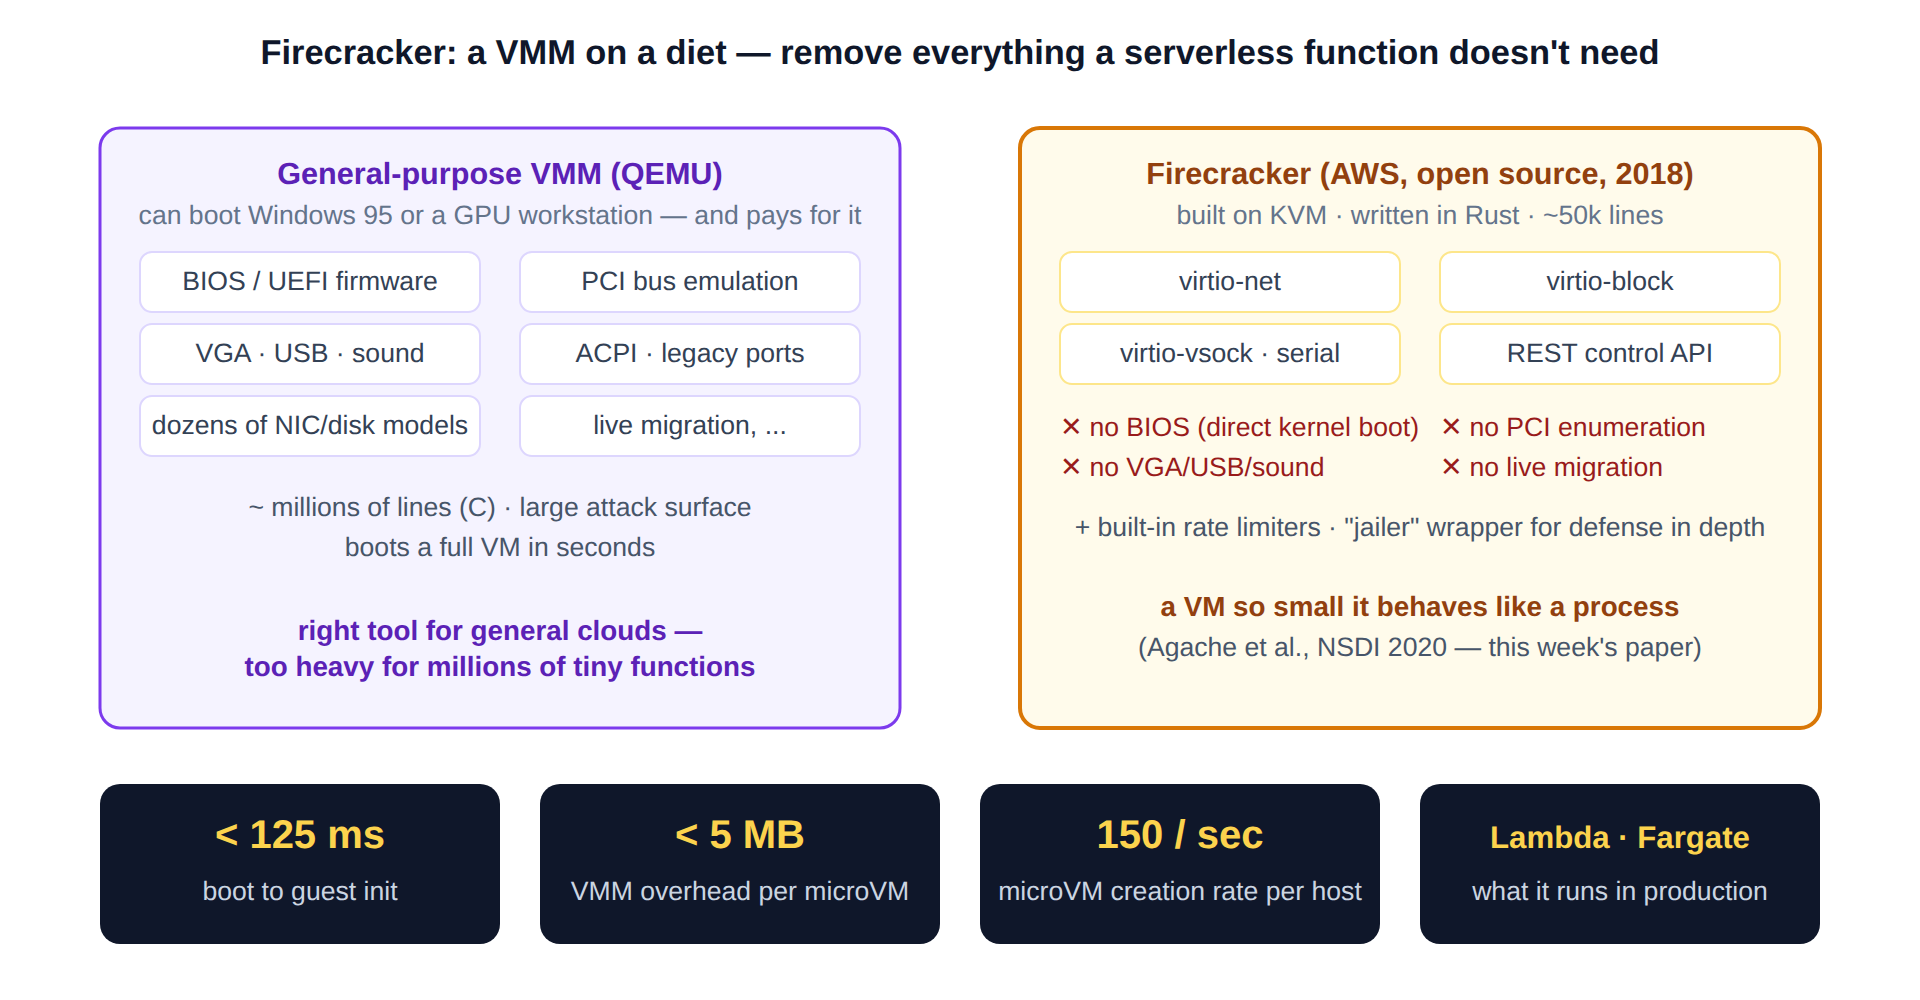
\includegraphics{figures/fig2-6_firecracker.png}}\\[3pt]
  \figcaption{그림 2-6  Firecracker: KVM은 유지하고 장치 박물관은 없앤다. 125 ms, 5 MB, 150/s라는 수치는 이번 주 필독 자료인 NSDI 2020 논문에서 가져왔다.}
\end{tbbfigure}

\begin{tbbtablewrap}
  \begin{tabular}{@{}>{\raggedright\arraybackslash}m{\dimexpr 0.2021\tbltextwidth-2\tabcolsep\relax} >{\raggedright\arraybackslash}m{\dimexpr 0.1968\tbltextwidth-2\tabcolsep\relax} >{\raggedright\arraybackslash}m{\dimexpr 0.1968\tbltextwidth-2\tabcolsep\relax} >{\raggedright\arraybackslash}m{\dimexpr 0.2021\tbltextwidth-2\tabcolsep\relax} >{\raggedright\arraybackslash}m{\dimexpr 0.2021\tbltextwidth-2\tabcolsep\relax}@{}}
  \arrayrulecolor{tbbnavy}\specialrule{1pt}{0pt}{0pt}
  \rowcolor{tbbtablehead}{\centering \bfseries\color{tbbnavy} } & {\centering \bfseries\color{tbbnavy}컨테이너} & {\centering \bfseries\color{tbbnavy}gVisor} & {\centering \bfseries\color{tbbnavy}microVM (FC/Kata)} & {\centering \bfseries\color{tbbnavy}완전한 VM} \\
  \arrayrulecolor{tbbnavy}\specialrule{0.7pt}{0pt}{2pt}
  {\textbf{커널}} & {공유하는 호스트 커널} & {사용자 공간 프록시 커널} & {자체 게스트 커널} & {자체 게스트 커널} \\
  \arrayrulecolor{tbbtableborder}\hline
  {\textbf{격리 경계}} & {시스템 호출 인터페이스} & {Sentry + 축소한 시스템 호출} & {하드웨어(VT-x)} & {하드웨어(VT-x)} \\
  \arrayrulecolor{tbbtableborder}\hline
  {\textbf{시작 시간}} & {\textasciitilde{}100 ms} & {\textasciitilde{}100 ms} & {\textasciitilde{}125 ms–1 s} & {초–분} \\
  \arrayrulecolor{tbbtableborder}\hline
  {\textbf{인스턴스당 오버헤드}} & {≈ 0} & {시스템 호출 비용} & {\textasciitilde{}5 MB + 게스트 커널} & {수백 MB} \\
  \arrayrulecolor{tbbtableborder}\hline
  {\textbf{일반적인 용도}} & {자체 워크로드, K8s 기본값} & {멀티테넌트 PaaS (Google)} & {FaaS, 신뢰할 수 없는 코드(AWS)} & {임대한 클라우드 서버} \\
  \arrayrulecolor{tbbnavy}\specialrule{1pt}{2pt}{0pt}
  \end{tabular}\par
  \figcaption{표 2-2  격리 선택지 비교(벤치마크가 아닌 규모 차수)}
\end{tbbtablewrap}

\subsection*{서빙에 주는 의미(12주 차로 이어지는 실마리)}

이를 제1장의 0으로 스케일링 이야기와 연결하면 그림이 유용하게 선명해진다. Firecracker는 \textit{환경}이 \textasciitilde{}125 ms 안에 나타날 수 있음을 입증한다. 따라서 GPU 기반 모델 엔드포인트의 콜드 스타트가 30–60 s라면 microVM이 범인이 아니다. GPU 호스트를 스케줄링하고, 수 기가바이트 컨테이너 이미지를 가져오며, 수십 기가바이트 가중치를 GPU 메모리에 로드하고, 런타임 캐시를 워밍업하는 데 시간이 쓰였다. 이 분해 자체가 12주 차 수업의 씨앗이다. 가상화는 제 몫을 다했고, 남은 콜드 스타트 엔지니어링은 이미지, 가중치, GPU 상태에 관한 것이다. 그래서 \textit{로드된} VM의 스냅숏/복원 같은 기법(Firecracker 스냅숏은 현재 서버리스 GPU 연구와 실무의 한 흐름이다)이 최전선에 있다. 이제 서버리스 GPU 플랫폼이 콜드 스타트 수치를 제시하면 그 수치를 검증할 방법을 안다.

\begin{calloutbox}{tbbpurple}{tbbpurplefill}
{\normalsize\bfseries\color{tbbpurple}생각해 보기}\par\vspace{3pt}
\begin{tbbitemize}
  \item 팀이 AI 에이전트 제품에서 모델이 생성한 신뢰할 수 없는 Python을 실행한다고 하자. 커널 0-day의 피해 범위, 시작 지연 시간 예산(대화형이다!), 호스트당 밀도, GPU 접근(2.6절을 미리 보자)을 기준으로 이 샌드박스에 컨테이너, gVisor, Firecracker 중 무엇이 적합한지 논증해 보자.
  \item 밀도를 계산해 보자. 호스트에 테넌트용 RAM 384 GB가 있다. 유휴 상태인 128 MB 힙을 쓰는 함수가 (a) 컨테이너(\textasciitilde{}0 오버헤드), (b) Firecracker microVM(각각 +5 MB + \textasciitilde{}20 MB 게스트 커널), (c) 완전한 VM(각각 +300 MB)에 몇 개씩 들어가는지 추정하라. 그 결과는 호출당 가격에 어떤 영향을 주는가?
\end{tbbitemize}
\end{calloutbox}

\section{클라우드의 GPU: 인스턴스, 패스스루, 공유}

지금까지 이 장에서는 CPU, 메모리, I/O를 가상화했다. 이제 이 과정의 실제 중심인 구성 요소를 더해 보자. GPU는 앞의 모든 방법론에 완강히 저항한다. "GPU용 VT-x"는 없다. 아키텍처의 non-root 모드도, CUDA용 하드웨어 트랩 후 에뮬레이션도 없다. GPU는 마이크로초 만에 세계 전환할 수 없는 수 기가바이트의 컨텍스트를 보관하고, 거대한 독점 드라이버 스택으로 구동되며, 정중한 시분할이 아니라 까다로운 소유자 한 명을 위해 설계되었다. 따라서 "테넌트가 GPU를 어떻게 얻는가?"에 대한 클라우드의 답은 앞의 모든 것과 다르다. 세 가지 답(그림 2-7)은 12주 차까지 따라다닌다. \textbf{GPU를 얼마나 세밀하게 공유할 수 있는가는 가상화 의상을 입은 서빙 경제성 문제}이기 때문이다.

\subsection*{먼저 가격표의 형태: GPU 인스턴스 계열}

공급자는 제1장의 학습과 추론 구분을 반영한 인스턴스 계열로 GPU를 패키징한다. \textbf{학습형 인스턴스}는 플래그십 가속기(H100/H200/B200급) 8개를 한 섀시에 넣고 내부는 NVLink, 섀시 사이는 매우 빠른 패브릭으로 연결한다. AWS P 계열, GCP A3, Azure ND 계열이 있다. \textbf{추론형 인스턴스}는 적당한 CPU 수에 소형 GPU(T4, L4, A10급) 하나에서 몇 개를 연결한다. AWS G 계열, GCP G2가 있으며 시간당 비용이 약 10배 낮다. 이 과정의 실습도 이 범위에서 진행한다(AWS g4dn 같은 T4 인스턴스나 GCP N1+T4 조합). 초보자를 놀라게 하는 실용적인 주의 사항이 두 가지 있다. GPU 인스턴스는 흔히 \textbf{할당량으로 잠겨} 있어 시작 전에 접근을 요청해야 하므로 실습 초반에 신청해야 한다. 또한 제1장의 메모리 적합성 계산에 따라 이 과정에서는 GPU 사양표보다 \textbf{VRAM}이 더 중요하다.

\begin{tbbtablewrap}
  \begin{tabular}{@{}>{\raggedright\arraybackslash}m{\dimexpr 0.1862\tbltextwidth-2\tabcolsep\relax} >{\raggedright\arraybackslash}m{\dimexpr 0.2660\tbltextwidth-2\tabcolsep\relax} >{\raggedright\arraybackslash}m{\dimexpr 0.1915\tbltextwidth-2\tabcolsep\relax} >{\raggedright\arraybackslash}m{\dimexpr 0.3564\tbltextwidth-2\tabcolsep\relax}@{}}
  \arrayrulecolor{tbbnavy}\specialrule{1pt}{0pt}{0pt}
  \rowcolor{tbbtablehead}{\centering \bfseries\color{tbbnavy}GPU (VRAM)} & {\centering \bfseries\color{tbbnavy}대표 인스턴스} & {\centering \bfseries\color{tbbnavy}대략적인 \$/hr} & {\centering \bfseries\color{tbbnavy}서빙 최적 용도} \\
  \arrayrulecolor{tbbnavy}\specialrule{0.7pt}{0pt}{2pt}
  {\textbf{T4 (16 GB)}} & {AWS g4dn.xlarge · GCP N1+T4} & {≈ \$0.5} & {이 과정의 실습 기준, 소형 모델, INT8 추론} \\
  \arrayrulecolor{tbbtableborder}\hline
  {\textbf{L4 (24 GB)}} & {GCP g2-standard-4 · AWS g6} & {≈ \$0.7–1.0} & {현대 추론의 주력, 토큰당 낮은 전력} \\
  \arrayrulecolor{tbbtableborder}\hline
  {\textbf{A10G (24 GB)}} & {AWS g5.xlarge} & {≈ \$1.0} & {중형 모델 — 제1장 사례 1-B에서 사용} \\
  \arrayrulecolor{tbbtableborder}\hline
  {\textbf{A100 (80 GB)}} & {AWS p4d (÷8) · GCP a2} & {GPU당 ≈ \$3–5} & {대형 모델(양자화 70B), 분할용 MIG 호스트(아래 절)} \\
  \arrayrulecolor{tbbtableborder}\hline
  {\textbf{H100 (80 GB)}} & {AWS p5 (÷8) · GCP a3} & {GPU당 \$2–7(채널에 따라 다름)} & {프런티어 서빙 및 학습, NVLink 연결} \\
  \arrayrulecolor{tbbtableborder}\hline
  {\textcolor{tbbgray}{(참고) B200 (192 GB)}} & {\textcolor{tbbgray}{차세대}} & {\textcolor{tbbgray}{\$4–6+}} & {\textcolor{tbbgray}{GPU당 상한을 다시 높임}} \\
  \arrayrulecolor{tbbnavy}\specialrule{1pt}{2pt}{0pt}
  \end{tabular}\par
  \figcaption{표 2-3  서빙 서버군의 가격(2026년 중반의 온디맨드 예시 — 숫자보다 구조가 오래간다)}
\end{tbbtablewrap}

제1장의 두 관점으로 이 표를 읽으면 목록이 아니라 의사 결정 도구가 된다. \textbf{결정적인 제약 차원:} 양자화 모델에 11 GB가 필요하다면 T4와 그 위의 모든 GPU가 \textit{작동}하지만, T4에서 L4 사이만 \textit{경제적}이다. T4 경제성으로 모델을 검증하고 "안전을 위해" A100에 배포하면 제약이 되지 않는 VRAM과 FLOPs에 시간당 6–10×를 지불한다. \textbf{사용률:} 서빙하든 놀든 가격 열의 요금이 시간당 부과되므로, 서버군에 관한 질문은 "어느 GPU가 가장 좋은가?"가 아니라 "실제로 유지할 수 있는 사용률에서 SLO를 충족하는 가장 저렴한 카드는 무엇인가?"다. 12주 차에는 오토스케일링과 GPU 공유가 이 표를 최적화 문제로 바꾼다. \textit{서버군 표}로 기억하자.

\subsection*{VM이 GPU 전체를 얻는 방법: PCIe 패스스루}

\begin{terminalbox}
\begin{Verbatim}[breaklines=true,breakanywhere=true,fontsize=\small,formatcom=\color{tbbtermfg},codes=\tbbcodeactive]
# on this week's rented VM - recall Exhibit 2-A: everything so far was fake
$ lspci | grep -i nvidia
00:1e.0 3D controller: NVIDIA Corporation TU104GL [Tesla T4]
$ nvidia-smi --query-gpu=name,driver_version,memory.total --format=csv
name, driver_version, memory.total [MiB]
Tesla T4, 550.54.15, 16384 MiB
# a REAL PCI device, running the REAL driver, inside the fake machine.
# the one component the hypervisor did not fake. how? and why not?
\end{Verbatim}
\end{terminalbox}
\figcaption{기록 2-4  환상 속의 예외. 디스크는 virtio, 시계는 kvm-clock, CPU 모델은 메뉴에서 고른 것이지만 T4는 패스스루된 물리 실리콘이다. 이 하위 절에서는 그 방법(VFIO + IOMMU)과 대가(카드당 테넌트 하나)를 설명한다.}

이번 주 g4dn을 시작했을 때 \code{nvidia-smi}에 보이는 T4는 에뮬레이션이나 프록시가 아니라 \textbf{물리 카드}다. 메커니즘은 \textbf{PCIe 패스스루}다. 호스트가 Linux VFIO 프레임워크를 통해 장치를 자신에게서 분리해 게스트에 매핑한다. 게스트는 실제 NVIDIA 드라이버를 로드하고 실제 실리콘과 통신한다. 이를 가능하게 하는 하드웨어는 표 2-1의 \textbf{IOMMU}(Intel VT-d / AMD-Vi)다. GPU는 메모리를 직접 읽고 쓰는 DMA 엔진이므로, 통제되지 않은 DMA 엔진을 테넌트에 넘기면 호스트 전체를 읽을 수 있다. IOMMU는 장치에 자체 주소 변환을 제공한다. 게스트 메모리 접근이 EPT를 통과하듯 DMA 주소도 하이퍼바이저가 제어하는 테이블을 통과하므로, GPU는 자기 게스트의 페이지만 건드릴 수 있다. 패스스루 덕분에 클라우드 GPU는 네이티브에 가까운 성능을 낸다. 설정 후 데이터 경로에는 하이퍼바이저가 전혀 관여하지 않는다. 한계도 마찬가지로 구조적이다. \textbf{할당 단위가 물리 GPU 하나 전체}다. 테넌트 하나, 카드 하나이므로 중재할 것이 없다. (VM이 호스트에 고정되기도 한다. 패스스루 장치를 사용하면 라이브 마이그레이션할 수 없어서 GPU 인스턴스가 유지보수 때 이동하지 않고 중단되는 이유 중 하나다.)

\subsection*{GPU 하나 공유하기: 시간 분할, vGPU, MPS, MIG}

모델이 작아지는 순간 GPU 전체 할당은 제1장의 사용률 문제와 충돌한다. 80 GB H100에서 3 GB 모델을 실행하면 랙에서 가장 비싼 부품의 96\%를 낭비한다. 공유 선택지는 \textit{무엇이 공정성을 강제하는지}에 따라 나뉜다. 소프트웨어 스케줄인지 실리콘 파티션인지가 차이다(그림 2-7).

\begin{tbbfigure}
  \adjustbox{max width=0.94\linewidth,max totalheight=0.46\textheight}{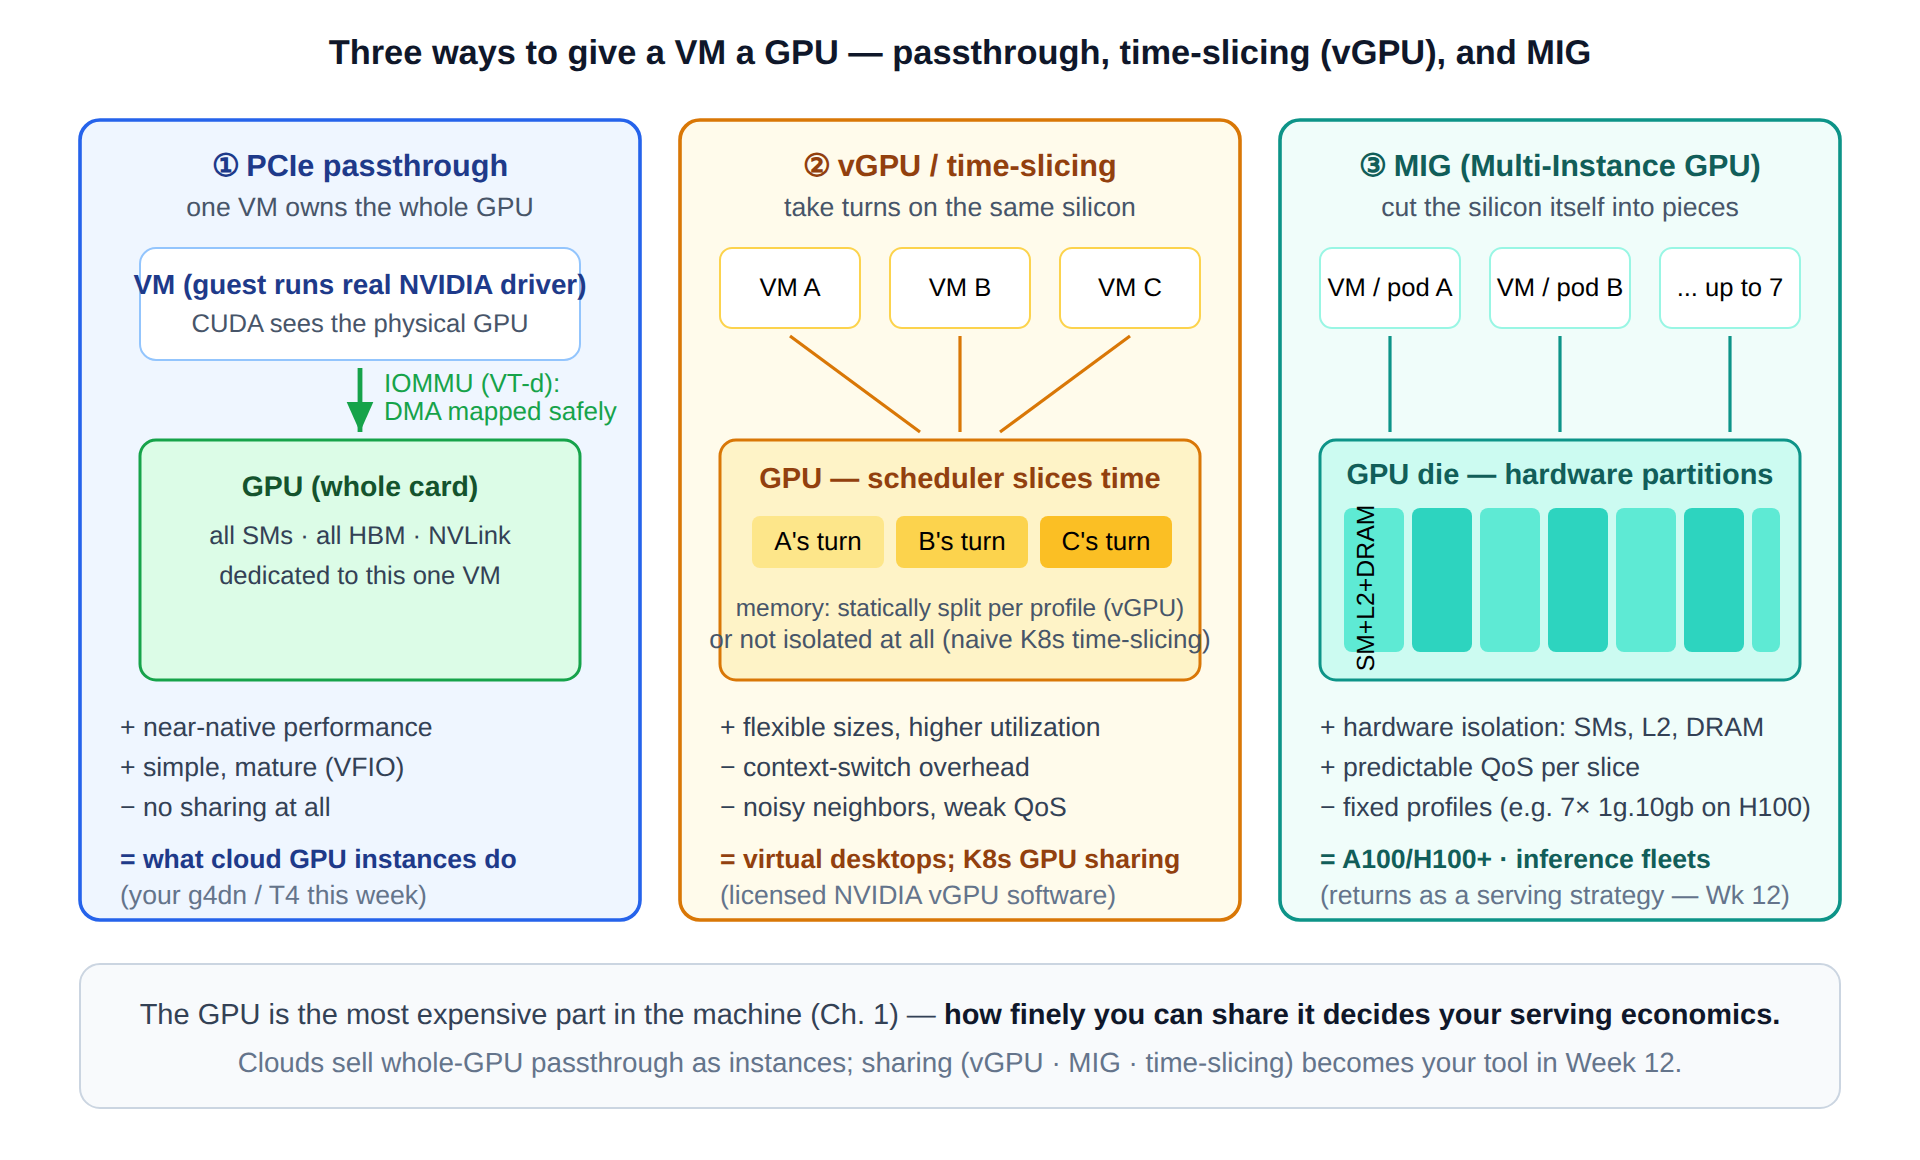
\includegraphics{figures/fig2-7_gpu_virt.png}}\\[3pt]
  \figcaption{그림 2-7  GPU에 접근하는 세 가지 방식. 인스턴스가 판매하는 독점 패스스루, 시간적 공유(vGPU/시간 분할/MPS), 공간적 하드웨어 파티셔닝(MIG)이다.}
\end{tbbfigure}

\begin{tbbitemize}
  \item \textbf{단순 시간 분할}(Kubernetes GPU 시간 분할 등)은 여러 워크로드가 번갈아 같은 GPU에 작업을 제출하게 한다. 메모리를 나누는 것도, 차례의 공정성을 보장하는 것도 없다. 테넌트 하나가 VRAM 전체를 할당하거나 긴 커널을 독점할 수 있다. 신뢰하고 협력하는 작업 사이에서는 쓸 만하지만, 낯선 사용자나 꼬리 지연 시간 약속에는 적합하지 않다.
  \item \textbf{NVIDIA vGPU}는 VM의 시간적 공유를 제품화한다. 라이선스가 필요한 호스트 소프트웨어와 \textit{VRAM을 정적으로 나누는} 프로필을 사용해 각 vGPU가 자기 조각을 소유하며, 스케줄러가 거의 일반적인 드라이버를 실행하는 게스트 사이에서 계산 시간을 분할한다. 가상 데스크톱용으로 탄생했지만 추론에도 쓸 수 있다. 계산 QoS는 여전히 하드웨어급이 아니라 스케줄러급이다.
  \item \textbf{MPS (Multi-Process Service)}는 한 소유자의 프로세스 \textit{내에서} CUDA 수준으로 공유한다. 프로세스 여러 개의 커널이 GPU 하나에서 동시에 실행되며 선택적으로 자원 한도를 둘 수 있다. 자체 모델을 함께 배치하기에는 훌륭하지만 보안 경계는 전혀 제공하지 않는다.
  \item \textbf{MIG (Multi-Instance GPU}, Ampere/A100 이후\textbf{)}는 마침내 CPU가 2005년에 한 일을 수행한다. 격리를 실리콘 안으로 옮긴다. 다이는 최대 \textbf{7개 인스턴스}로 분할되며 각 인스턴스가 자체 SM 조각, L2 조각, DRAM 컨트롤러/용량을 소유한다. 예를 들어 H100-80GB 한 대에서 1g.10gb 인스턴스 7개를 만들거나 3g.40gb + 2g.20gb + 2g.20gb처럼 크기를 섞을 수 있다. 각 인스턴스에는 하드웨어가 강제하는 메모리 대역폭과 용량이 있으므로 이웃이 난동을 부려도 지연 시간이 움직이지 않는다. 서빙 서버군이 갈망하는 \textbf{조각별 예측 가능한 p99}를 제공한다. 대가는 고정된 프로필 메뉴, 하나의 작업에 협력하지 못하는 인스턴스, 중단을 일으키는 재구성이다. 보장을 얻기 위해 경직성을 감수하는 절충이며 12주 차에 가격을 계산한다.
\end{tbbitemize}

\begin{tbbtablewrap}
  \begin{tabular}{@{}>{\raggedright\arraybackslash}m{\dimexpr 0.2181\tbltextwidth-2\tabcolsep\relax} >{\raggedright\arraybackslash}m{\dimexpr 0.1915\tbltextwidth-2\tabcolsep\relax} >{\raggedright\arraybackslash}m{\dimexpr 0.1862\tbltextwidth-2\tabcolsep\relax} >{\raggedright\arraybackslash}m{\dimexpr 0.1809\tbltextwidth-2\tabcolsep\relax} >{\raggedright\arraybackslash}m{\dimexpr 0.2234\tbltextwidth-2\tabcolsep\relax}@{}}
  \arrayrulecolor{tbbnavy}\specialrule{1pt}{0pt}{0pt}
  \rowcolor{tbbtablehead}{\centering \bfseries\color{tbbnavy} } & {\centering \bfseries\color{tbbnavy}시간 분할(K8s)} & {\centering \bfseries\color{tbbnavy}NVIDIA vGPU} & {\centering \bfseries\color{tbbnavy}MPS} & {\centering \bfseries\color{tbbnavy}MIG} \\
  \arrayrulecolor{tbbnavy}\specialrule{0.7pt}{0pt}{2pt}
  {\textbf{공유 유형}} & {시간적} & {시간적 + 정적 VRAM} & {동시 실행(CUDA)} & {공간적(하드웨어)} \\
  \arrayrulecolor{tbbtableborder}\hline
  {\textbf{메모리 격리}} & {없음} & {정적 파티션} & {없음} & {하드웨어 강제} \\
  \arrayrulecolor{tbbtableborder}\hline
  {\textbf{QoS / p99}} & {없음} & {스케줄러급} & {한도, 경계 없음} & {하드웨어급} \\
  \arrayrulecolor{tbbtableborder}\hline
  {\textbf{보안 경계}} & {없음} & {VM급(라이선스)} & {없음} & {있음(인스턴스별)} \\
  \arrayrulecolor{tbbtableborder}\hline
  {\textbf{최적 용도}} & {신뢰하는 배치 작업} & {VDI, 혼합 VM} & {함께 배치한 자체 모델} & {멀티테넌트 추론} \\
  \arrayrulecolor{tbbnavy}\specialrule{1pt}{2pt}{0pt}
  \end{tabular}\par
  \figcaption{표 2-4  GPU 공유 선택지 한눈에 보기}
\end{tbbtablewrap}

마지막 연결점을 보자. GPU는 이 장에서 CPU의 역사 전체를 되풀이했다. 가상화 이전 서버 같은 독점 소유, 바이너리 변환 시대처럼 보장이 약한 소프트웨어 시분할, 그리고 하드웨어가 강제하는 파티션으로 이어졌다. MIG는 GPU의 VT-x 순간이다. 아키텍처에는 운율이 있다.

\begin{calloutbox}{tbbpurple}{tbbpurplefill}
{\normalsize\bfseries\color{tbbpurple}생각해 보기}\par\vspace{3pt}
\begin{tbbitemize}
  \item 내부 추론 서비스 세 개가 각각 \textasciitilde{}15 GB VRAM과 p99 SLO를 필요로 한다. H100-80GB 한 대가 있다. MIG 프로필, MPS, 별도의 L4 인스턴스 세 대를 격리, 사용률, 비용, 장애 피해 범위 관점에서 비교해 논증하라.
  \item 패스스루는 라이브 마이그레이션을 막지만 virtio 장치는 막지 않는 이유는 무엇인가? (각 경우에 상태가 어디에 존재하는지 생각해 보자.)
\end{tbbitemize}
\end{calloutbox}

\section{실습: 첫 클라우드 GPU를 안전하게 사용하기}

실습은 이 장을 구체화한다. 클라우드 계정을 만들고 \textbf{무엇보다 먼저 과금 안전장치를 설정}한 뒤 GPU VM을 시작한다. \code{nvidia-smi}로 하드웨어를 만나고, 같은 추론 작업에서 CPU와 GPU의 속도를 겨루며, 계량기를 켜 둔 채 남기지 않고 모두 종료한다. 클릭 단위의 자세한 절차는 실습 안내서에 있다. 콘솔은 교재보다 빨리 바뀌기 때문이다. 여기서는 각 단계의 \textit{이유}와 예상할 수치를 다룬다. 산출물은 측정한 지연 시간과 이 장에 연결한 관찰 세 가지를 담은 1쪽 보고서다.

\subsection*{0단계 — 계산 자원보다 먼저 비용 안전장치}

제1장은 "시간당 과금 = 유휴 시간은 돈"이라는 말로 끝났다. 여기서 이를 몸에 익힌다. 무엇이든 시작하기 전에 \textbf{(a)} 공급자 과금 콘솔에서 알림 임계값이 있는 예산(예: \$10의 50/80/100\%에서 이메일)을 만들고, \textbf{(b)} 교육용 크레딧을 사용 중이며 계량값이 어디에 표시되는지 확인하고, \textbf{(c)} 두 시계를 이해해야 한다. \textit{중지한} 인스턴스는 계산 요금이 멈추지만 \textbf{연결된 디스크 스토리지 요금은 계속 부과}된다. \textit{종료한} 인스턴스는 모든 자원과 별도 지시가 없다면 디스크도 해제한다. 초보자의 전형적인 청구서는 GPU 시간 때문이 아니다. 오래 중지한 인스턴스에 연결한 채 잊은 200 GB 볼륨이나, 버려진 브라우저 탭에서만 "중지"한 인스턴스 때문이다. 실습 체크리스트의 마지막은 콘솔에 \textbf{실행 중인 인스턴스 0개, 연결되지 않은 볼륨 0개}가 표시되는지 확인하는 것이다. 보고서용으로 화면을 캡처한다.

\subsection*{1\textasciitilde{}3단계 — 할당량, 시작, GPU 만나기}

GPU 할당량은 일찍 요청한다. 승인에 몇 시간이 걸릴 수 있다. 가까운 리전에서 가장 저렴한 T4 인스턴스 유형(AWS \code{g4dn.xlarge} 또는 GCP N1 + T4급, 시간당 약 1달러)를 고른다. 측정 자체에는 계정 없이 쓸 수 있는 대안으로 Colab이 있다. 드라이버가 사전 설치된 딥러닝 OS 이미지를 선택하고 ssh로 접속한다. 그런 다음 시스템 관점에서 \code{nvidia-smi}를 읽어 보자. 모든 필드가 이 장의 내용을 되풀이한다. \textbf{드라이버/CUDA 버전}은 \textit{게스트}에 속한다. T4가 \textbf{패스스루}되었으므로 VM이 실제 드라이버를 실행한다(§2.6). \textbf{메모리 표시값(0/16384 MiB)}은 제1장의 계산과 10주 차의 양자화가 관리할 VRAM 예산이다. \textbf{사용률과 프로세스 목록}은 12주 차 오토스케일러와 14주 차 대시보드가 소비할 메트릭이다. \code{lspci | grep -i nvidia}도 실행한다. GPU가 물리 카드처럼 게스트 PCI 버스에 있으며, 패스스루가 눈에 보인다. 40초 동안의 시작이 기계적으로 무엇이었는지도 주목하자. 컨트롤 플레인이 호스트를 골랐고, 하이퍼바이저(이 장)가 게스트를 구체화했으며, 펌웨어가 없거나 빠른 부팅이 커널을 올렸고, cloud-init이 개인화했다. 이제 콜드 스타트를 직접 눈으로 보았다. 12주 차에는 이 관찰을 산업 규모로 확장한다.

\subsection*{4단계 — 측정: CPU 추론 대 GPU 추론}

안내서의 벤치마크 스크립트를 실행한다. 소형 트랜스포머(DistilBERT급)나 소형 CNN에 같은 입력 배치를 넣고 CPU와 GPU에서 시간을 잰다. PyTorch에서는 \code{.to("cuda")} 하나가 차이다. 코드보다 프로토콜이 중요하다. \textbf{먼저 워밍업하라.} 첫 GPU 호출에는 CUDA 컨텍스트, 메모리 풀, 커널 선택 같은 일회성 비용이 들어 CPU보다 \textit{느릴 수도 있다}. 개인적으로 얻은 첫 콜드 스타트 데이터로 따로 보고하고, 이후 약 100회의 정상 상태 시간을 측정한다. 배치 크기(1, 8, 32, 64)를 바꾸며 \textbf{배치당 지연 시간과 처리량}을 모두 기록한다. 결과의 대략적인 규모는 다음과 같을 것이다. CPU는 배치 크기 1에서 수십 ms이며 배치에 따라 거의 선형으로 증가한다. GPU는 배치 크기 1에서 수 ms이고, 배치가 커져도 \textit{거의 움직이지 않다가} 배치 크기 32–64에서 처리량이 CPU의 10–50×가 된다. GPU의 배치 크기 1 성능이 기대에 못 미친다면 이유를 다시 발견한 것이다. 작은 작업에서는 시작 오버헤드와 PCIe 홉이 지배하며, 병렬 하드웨어는 폭넓게 일을 줄 때 값을 한다. 제1장의 처리량과 지연 시간 사이 긴장, 그리고 10주 차 배칭의 전체 동기를 직접 측정한 셈이다. 보고서에 바로 이런 관찰을 적어야 한다.

\begin{calloutbox}{tbbpurple}{tbbpurplefill}
{\normalsize\bfseries\color{tbbpurple}실습 체크리스트(크레딧을 지키는 버전)}\par\vspace{3pt}
\begin{tbbitemize}
  \item 첫 시작 \textbf{전에} 예산 + 알림이 존재하며, 과금 페이지 위치를 안다.
  \item GPU 할당량을 일찍 요청하고, 가장 저렴한 T4 인스턴스 유형, 가까운 리전, 드라이버가 포함된 딥러닝 이미지를 선택한다.
  \item \code{nvidia-smi}와 \code{lspci} 출력을 저장하고, 워밍업과 정상 상태를 따로 측정하며, 배치 변화(1/8/32/64)를 기록한다.
  \item 이유가 없다면 인스턴스를 단순히 중지하지 않고 \textbf{종료}한다. 볼륨을 확인하고, 실행 중이거나 고아가 된 자원이 없는 최종 콘솔 화면을 캡처한다.
  \item 보고서에는 수치와 §2.3–§2.6에 연결한 관찰 세 가지를 담는다(예: 스틸 타임을 보았는가? 워밍업 비용은? 배치 효과는?).
\end{tbbitemize}
\end{calloutbox}

\vspace{3.0pt}

\begin{calloutbox}{tbbpurple}{tbbpurplefill}
{\normalsize\bfseries\color{tbbpurple}생각해 보기}\par\vspace{3pt}
\begin{tbbitemize}
  \item 배치 크기 1의 GPU 지연 시간은 CPU보다 거의 빠르지 않지만, 배치 크기 64의 GPU 처리량은 CPU의 40×다. 프로덕션 트래픽은 한 번에 요청 하나씩 도착한다. 어떤 선택지가 있는가? (방금 10\textasciitilde{}12주 차의 의제를 다시 발명했다.)
  \item g4dn.xlarge가 \$0.53/hr일 때 효율적으로 2시간 작업하면 실습 전체 비용이 얼마인지 추정해 보자. 인스턴스를 한 달 동안 잊으면 얼마인가? 안전장치는 어느 숫자를 막으려 하는가?
\end{tbbitemize}
\end{calloutbox}

\namedsection{요약}{열두 가지로 정리한 제2장}

\qitem{1}{\textbf{임대한 머신은 존재하지 않으며, 스스로 그렇게 말한다.} 하이퍼바이저(VMM)는 물리 호스트 하나를 격리된 가상 머신 여러 개로 다중화한다. 게스트는 소매업체 이름이 들어간 DMI 문자열, \code{kvm}이라고 답하는 \code{systemd-detect-virt}, \code{kvm-clock}으로 도착하는 시계에서 직접 자백을 읽을 수 있다(사례 2-A). 이 소프트웨어 환상이 시간당 과금, 멀티테넌시, 탄력성의 기반이다.}

\qitem{2}{\textbf{가상화는 "비싼 하드웨어가 놀고 있다"는 질문에 대한 60년 된 답이다.} 1막: 수백만 달러짜리 메인프레임 → 시분할과 CP-67의 사용자별 가상 머신(1967). 2막: 5–15\% 사용률로 난립한 2000년대 서버 → VMware 통합. 3막: EC2의 \textit{시간당 \$0.10}(2006). 할당이 소프트웨어가 되면서 계산 자원에 계량기가 생겼다. GPU는 다시 1막을 살고 있으며, §2.6은 진행 중인 GPU의 2막과 3막이다.}

\qitem{3}{\textbf{Popek \& Goldberg (1974)}는 동등성, 효율성, 자원 제어라는 계약과 정리를 정의했다. 모든 민감 명령어가 특권 명령어, 즉 트랩하는 명령어일 때만 트랩 후 에뮬레이션이 작동한다. 고전적 x86에는 민감하지만 특권은 아닌 명령어 17개가 있어 이 조건을 깨뜨렸다.}

\qitem{4}{두 소프트웨어 시대의 기법이 간극을 메웠다. \textbf{바이너리 변환}(VMware)은 게스트를 실행 중에 다시 써서 수정하지 않은 게스트를 완전 가상화했고, \textbf{반가상화}(Xen)는 게스트를 수정해 하이퍼콜을 사용함으로써 소스가 필요하지만 더 빠르게 실행했다. 협력하는 게스트라는 아이디어는 오늘날 virtio로 살아 있다.}

\qitem{5}{\textbf{VT-x/AMD-V (2005–06)}는 VMCS를 계약으로 삼아 VMX root/non-root 모드를 추가했다. 게스트 커널은 다시 ring 0에서 실행되고 위험한 작업은 하드웨어 VM exit를 일으킨다. \textbf{Exit는 가상화 성능의 통화}이므로 횟수를 세고 비용을 낮춰야 한다.}

\qitem{6}{\textbf{EPT/NPT}는 섀도 페이지 테이블을 끝냈다. 하드웨어가 두 변환(guest VA → guest PA → host PA)을 순회한다. 비용은 더 무거운 TLB 미스로 드러나므로 대형 페이지가 중요하며, 메모리를 많이 쓰는 추론에서는 특히 그렇다.}

\qitem{7}{\textbf{KVM + QEMU + virtio}는 하이퍼바이저가 된 Linux다. KVM은 커널에서 VT-x를 구동하고, QEMU는 VM별 장치 모델을 제공하며, virtio는 장치의 환상을 exit마다 작업을 배치하는 정직한 공유 메모리 virtqueue로 대체한다. \textbf{vCPU는 그저 호스트 스레드}이므로 오버커밋과 스틸 타임, 그리고 꼬리 지연 시간에 미치는 영향이 따라온다.}

\qitem{8}{\textbf{격리 스펙트럼}은 테넌트 코드와 호스트 커널 사이에 무엇이 있는지에 따라 선택지를 나열한다. 프로세스 < 컨테이너(공유 커널!) < gVisor(사용자 공간 커널) < microVM < 완전한 VM 순이며, 시작 시간과 밀도를 격리 강도와 교환한다.}

\qitem{9}{\textbf{Firecracker}는 서버리스 시대의 답이다. KVM은 유지하고 장치 박물관은 없앤다. <125 ms 부팅, <5 MB 오버헤드, 호스트당 150 microVMs/s로, 프로세스처럼 동작하며 Lambda와 Fargate를 실행하는 VM이다. 12주 차에 주는 교훈은 환경이 더는 콜드 스타트 병목이 아니며 이미지, 가중치, GPU 상태가 병목이라는 것이다.}

\qitem{10}{\textbf{GPU는 고전적 가상화에 저항하며} VT-x에 해당하는 기능이 없다. 따라서 클라우드는 카드 전체를 \textbf{PCIe 패스스루}한다(IOMMU/VFIO 사용, 네이티브에 가까운 성능, 공유 불가, 기록 2-4의 "가짜 머신 안의 진짜 카드"). 공유에는 \textbf{시간 분할/vGPU}(소프트웨어 공정성), \textbf{MPS}(함께 배치한 자체 워크로드), \textbf{MIG}(하드웨어 파티션, 최대 7개 격리 인스턴스와 조각별 메모리 및 예측 가능한 p99, GPU의 VT-x 순간)를 사용한다.}

\qitem{11}{\textbf{서버군 표(표 2-3)는 의사 결정 도구다.} 추론용 T4/L4/A10G의 \textasciitilde{}\$0.5–1.0/hr부터 GPU당 수 달러인 A100/H100까지 제시한다. "클수록 안전하다"는 목록으로 읽지 말고, 제1장의 결정적인 제약 차원(들어가면서 SLO를 충족하는 \textit{가장 저렴한} 카드는 무엇인가?)과 사용률 관점으로 읽어야 한다.}

\qitem{12}{\textbf{과금 안전장치는 엔지니어링 관행이다.} 처음 시작하기 전에 예산과 알림을 설정하고, 중지해도 무료가 아니며(디스크는 계속 과금된다), 종료하면 자원을 해제한다는 점을 이해한다. 실습은 빈 콘솔, 그리고 직접 측정한 첫 콜드 스타트와 CPU 대 GPU 배칭 곡선으로 끝난다.}

\namedsection{연습문제}{}

\subsection*{A. 객관식}

\qitem{1}{다음 중 Popek \& Goldberg가 제시한 가상 머신 모니터의 요구 사항이 아닌 것은?}

\begin{tbboptions}
  \item ① 동등성 — 게스트가 실제 하드웨어에서처럼 동작한다
  \item ② 효율성 — 대부분의 명령어가 CPU에서 직접 실행된다
  \item ③ 자원 제어 — VMM이 물리 자원을 완전히 통제한다
  \item ④ 이식성 — 어느 CPU 아키텍처에서든 게스트가 수정 없이 실행된다
\end{tbboptions}

\qitem{2}{VT-x에서 VMX non-root 모드로 실행되는 게스트 커널이 하이퍼바이저가 개입 대상으로 설정한 작업(예: I/O 포트 접근)을 실행하면 어떻게 되는가?}

\begin{tbboptions}
  \item ① 고전적 x86처럼 명령어가 조용히 아무 일도 하지 않는다
  \item ② 하드웨어가 VM exit를 수행한다. 게스트 상태를 VMCS에 저장하고 제어권을 root 모드의 하이퍼바이저로 넘긴다
  \item ③ 게스트 커널이 특권 폴트로 충돌한다
  \item ④ 명령어가 실행 중에 바이너리 변환된다
\end{tbboptions}

\qitem{3}{EPT/NPT가 해결하는 문제는?}

\begin{tbboptions}
  \item ① 게스트 물리 주소를 호스트 물리 주소로 하드웨어에서 변환하여 소프트웨어 섀도 페이지 테이블을 없앤다
  \item ② 하이퍼바이저로부터 게스트 메모리를 암호화한다
  \item ③ 게스트가 페이지 테이블을 공유하여 메모리를 절약하게 한다
  \item ④ 페이지 크기 전송으로 디스크 I/O를 가속한다
\end{tbboptions}

\qitem{4}{virtio 장치가 에뮬레이션 e1000 NIC보다 빠른 이유는?}

\begin{tbboptions}
  \item ① virtio 장치 코드가 더 빠른 언어로 작성되었다
  \item ② virtio 하드웨어가 e1000 하드웨어보다 물리적으로 새롭다
  \item ③ 게스트가 가상화 사실을 알고 협력한다. 공유 메모리 virtqueue를 통해 작업을 배치하므로 레지스터 접근마다 VM exit하는 대신 배치당 \textasciitilde{}한 번 exit한다
  \item ④ virtio는 모든 구성에서 커널을 완전히 우회한다
\end{tbboptions}

\qitem{5}{컨테이너와 (micro)VM 사이의 핵심 격리 차이는?}

\begin{tbboptions}
  \item ① 컨테이너는 CPU나 메모리 사용량을 제한할 수 없다
  \item ② 호스트의 컨테이너는 호스트 커널을 공유하므로 시스템 호출 인터페이스가 보안 경계다. 각 VM은 하드웨어 경계 뒤에 자체 커널을 둔다
  \item ③ VM에서는 Linux를 실행할 수 없다
  \item ④ 차이가 없으며 두 용어는 서로 바꿔 쓸 수 있다
\end{tbboptions}

\qitem{6}{테넌트별로 하드웨어가 강제하는 메모리와 대역폭 격리를 제공하는 GPU 공유 메커니즘은?}

\begin{tbboptions}
  \item ① Kubernetes 시간 분할        ② NVIDIA MPS
  \item ③ MIG (Multi-Instance GPU)      ④ CUDA 스트림
\end{tbboptions}

\qitem{7}{팀원이 말한다. "nvidia-smi에 실제 NVIDIA 드라이버를 사용하는 진짜 Tesla T4가 보이므로 EC2 인스턴스는 물리 서버임이 틀림없다." 올바른 반박은?}

\begin{tbboptions}
  \item ① 맞는 말이다. 실제 GPU가 있으면 실제 머신이다
  \item ② GPU는 디스크와 NIC처럼 QEMU가 에뮬레이션하므로 아무것도 증명하지 못한다
  \item ③ 머신은 KVM 게스트이며 dmidecode, systemd-detect-virt, kvm-clock이 모두 이를 증명한다. T4만 물리 장치이며 PCIe 패스스루로 통째로 매핑한, 환상에 대한 의도적 예외다
  \item ④ 가상 머신 안에서는 nvidia-smi를 전혀 실행할 수 없다
\end{tbboptions}

\subsection*{B. 단답형}

\qitem{1}{VT-x가 도입한 두 CPU 모드의 이름과 하이퍼바이저가 사용하는 모드를 쓰라.}

\qitem{2}{게스트 내부 모니터링에서 p99 지연 시간이 급증할 때 정확히 높은 \code{\%st}(스틸 타임)가 나타난다. 물리적으로 무슨 일이 일어나며 해결책 하나는 무엇인지 한 문장으로 설명하라.}

\qitem{3}{빈칸을 채워라. 물리 GPU를 게스트에 넘기는 것을 ( ㉠ )라 하며, 장치 DMA를 변환하고 통제하는 ( ㉡ ) 덕분에 안전하다.}

\qitem{4}{Firecracker는 microVM을 \textasciitilde{}125 ms에 부팅하지만 서버리스 GPU 모델 엔드포인트의 콜드 스타트에는 30초 이상이 걸릴 수 있다. 남은 시간이 쓰이는 곳 두 가지를 쓰라.}

\qitem{5}{양자화 모델에 VRAM 11 GB가 필요하고 L4(\textasciitilde{}\$0.8/hr)에서 SLO를 충족한다. 팀원이 "안전을 위해" A100-80GB(\textasciitilde{}\$4/hr)에 배포하자고 한다. 서버군 표가 이 제안에 적용하는 제1장의 두 관점을 각각 한 문장으로 설명하라.}

\subsection*{C. 서술형}

\qitem{1}{고전적 x86이 Popek \& Goldberg 정리에 따라 가상화할 수 없었던 이유를 설명하라. 바이너리 변환과 반가상화가 각각 어떻게 우회했는지 강점과 비용을 하나씩 들고, VT-x가 아키텍처 수준에서 문제를 해결한 방법을 설명하라.}

\qitem{2}{익명 사용자를 대신해 LLM이 작성한 코드를 실행하는 공개 "AI 에이전트" 서비스의 샌드박스를 설계한다. 격리 스펙트럼(컨테이너 / gVisor / Firecracker microVM / 완전한 VM)에서 한 지점을 선택하고, 커널 장애 피해 범위, 시작 지연 시간, 호스트당 밀도, 운영 복잡성을 고려해 양옆의 두 선택지보다 나은 이유를 논증하라.}

\qitem{3}{팀이 H100-80GB 한 대를 보유하고 있으며 p99 SLO가 있는 내부 모델 세 개(각각 \textasciitilde{}15 GB VRAM)와 카드 전체를 기꺼이 사용할 야간 배치 임베딩 작업을 실행해야 한다. MIG, MPS, 시간 분할, 시간대별 스케줄링을 자유롭게 조합해 GPU 공유 계획을 제안하고 격리, 사용률, 운영 단순성을 근거로 정당화하라. 계획 검증을 위해 무엇을 측정할지도 밝혀라.}

\namedsection{정답 및 해설}{}

\subsection*{A. 객관식}

\qitem{1}{\textbf{④} 세 요구 사항은 동등성, 효율성, 자원 제어다. 아키텍처 간 이식성은 포함되지 않는다. VMM은 자신이 실행되는 것과 \textit{같은} 아키텍처를 제공한다. (§2.2, 상자 2-1)}

\qitem{2}{\textbf{②} 정확히 VM exit다. 하드웨어가 게스트 상태를 VMCS에 저장하고 exit 이유를 기록한 뒤 root 모드로 진입한다. ①은 VT-x \textit{이전}의 병리 현상이고, ④는 소프트웨어 시대 VMware의 우회책이었다. (§2.3)}

\qitem{3}{\textbf{①} EPT/NPT는 CPU가 순회하는 두 번째 하이퍼바이저 소유 변환을 추가한다. 게스트는 exit 없이 자체 페이지 테이블을 관리하며 섀도 테이블은 사라진다. 비용은 TLB 미스 지연 시간으로 이동하므로 대형 페이지가 필요하다. (§2.3)}

\qitem{4}{\textbf{③} e1000 환상에서는 레지스터 접근마다 exit가 발생하지만, virtio의 정직한 인터페이스는 공유 링에 디스크립터를 배치하고 배치당 \textasciitilde{}한 번만 깨운다. 협력이 환상을 이긴다는 반가상화의 오래가는 교훈이다. (§2.4)}

\qitem{5}{\textbf{②} 컨테이너는 공유 커널 하나의 \textit{뷰}와 \textit{몫}을 격리한다(네임스페이스/cgroup, 제3장). VM은 테넌트와 호스트 사이에 하드웨어 경계와 비공개 커널을 둔다. 그림 2-5의 전체 축이 바로 이 차이다. (§2.5)}

\qitem{6}{\textbf{③} MIG만이 SM, L2, DRAM 등 실리콘 자체를 나누어 인스턴스별 하드웨어급 QoS를 제공한다. 시간 분할과 MPS는 하드웨어 경계 없이 시간적으로 또는 동시에 공유한다. (§2.6)}

\qitem{7}{\textbf{③} 사례 2-A의 증거(DMI 문자열, \code{systemd-detect-virt}, \code{kvm-clock})는 머신이 가상임을 입증한다. 기록 2-4는 그럼에도 GPU는 실제임을 보여 준다. VFIO/IOMMU를 통한 패스스루가 물리 카드를 게스트에 매핑한다. 가상 머신 안의 실제 장치는 모순이 아니라 의도한 결과다. (§2.1, §2.6)}

\subsection*{B. 단답형}

\qitem{1}{\textbf{VMX root 모드}(하이퍼바이저)와 \textbf{VMX non-root 모드}(게스트)다. 둘 다 rings 0–3을 포함하며, 게스트 커널은 하드웨어의 감독 아래 ring 0을 되찾는다.}

\qitem{2}{vCPU가 실행 가능할 때 호스트 스케줄러가 다른 테넌트의 스레드를 실행해 "CPU"가 보이지 않게 멈춘다. 전용 코어 인스턴스 유형을 쓰거나, 호스트당 vCPU를 줄여 오버커밋을 낮추거나, 지연 시간에 중요한 서빙을 공유 계열에서 옮길 수 있다.}

\qitem{3}{㉠ \textbf{PCIe 패스스루}(VFIO 사용), ㉡ \textbf{IOMMU}(Intel VT-d / AMD-Vi)다.}

\qitem{4}{GPU 호스트 스케줄링/탐색, 수 GB 컨테이너 이미지 가져오기, 수십 GB 모델 가중치를 GPU 메모리에 로드하기, CUDA/런타임 초기화와 캐시 워밍업 중 두 가지를 쓰면 된다. microVM 자체는 병목이 아니게 되었으며, 이것이 Firecracker의 성취이자 12주 차의 출발점이다.}

\qitem{5}{\textbf{결정적인 제약 차원:} 제약은 VRAM 11 GB이며 L4의 24 GB로 이미 충족한다. A100의 추가 56 GB와 FLOPs는 제약이 되지 않으므로 순수한 비용이다. \textbf{사용률/비용:} 계량기는 항상 시간당 돌아간다. 같은 SLO를 제공하면서 가격이 \textasciitilde{}5×면 요청당 비용은 \textasciitilde{}5× 늘고 비용을 낸 카드의 측정 사용률은 떨어진다. 여기서 "안전"은 "안전하게 낭비한다"는 뜻이다.}

\subsection*{C. 서술형(채점 기준)}

\qitem{1}{만점 답안에는 다음이 필요하다. 정리(민감 ⊆ 특권)와 이를 위반해 \textit{조용히} 실패하는 x86 명령어 17개(POPF가 대표 예시), 바이너리 변환 = 실행 중 게스트 커널 코드를 다시 쓰고 변환을 캐시(강점: 수정하지 않은 게스트, 비용: 엄청난 복잡성과 경계 사례), 반가상화 = 게스트 소스를 수정해 하이퍼콜(강점: 속도와 배칭, 비용: 게스트 변경이 필요하고 영구히 유지), VT-x = 직교하는 root/non-root 모드 + VMCS로 게스트에 ring 0을 돌려주고 모든 민감 작업이 하드웨어에서 확실히 트랩하게 함. virtio가 반가상화의 후손임을 언급하면 가산점이 있다. (§2.2–2.3)}

\qitem{2}{좋은 답은 \textbf{Firecracker형 microVM}을 선택하고 다음과 같이 논증한다. 커널 0-day에 대한 하드웨어 경계(공유 커널이나 Go 프록시가 상한인 컨테이너/gVisor와 대비), 대화형 예산 안의 \textasciitilde{}125 ms 부팅, 수천 개 밀도를 유지하는 \textasciitilde{}5 MB 오버헤드, 프로덕션 선례(Lambda)다. 컨테이너보다 구성 요소가 많고, 시스템 호출 호환성은 gVisor보다 단순하지만 장치/GPU 접근은 컨테이너보다 어렵다는 점도 솔직히 인정해야 한다. GPU 접근과 폭넓은 Linux 호환성이 중요하면 gVisor도 방어 가능한 대안이다. 선택한 브랜드가 아니라 \textit{절충에 대한 추론}을 평가한다. (§2.5)}

\qitem{3}{깔끔한 계획 하나는 H100을 SLO 서비스용으로 크기를 맞춘 격리 조각 세 개(예: 각각 2g.20gb ≈ 60 GB, p99용 하드웨어 QoS)로 MIG 파티셔닝하고, \textasciitilde{}1g.10gb는 오버플로/카나리용으로 남기는 것이다. 야간 배치 작업은 남은 조각에서 계속 실행하거나 한산한 시간에 \textit{재구성}해 실행한다. MIG 재구성은 중단을 일으키므로, 조각에서 MPS를 통해 배치 작업을 속도 제한하여 실행하는 방식과 비교해야 한다. 함께 배치했을 때와 격리했을 때의 서비스별 p99, 조각 사용률, 구성별 배치 작업 처리량을 반드시 측정해야 한다. 사용률과 격리의 대립이 하드웨어 조절 장치를 얻은 제1장의 비용 긴장임을 알아차린 답안에 가산점을 준다. (§2.6)}

\namedsection{더 읽을거리}{}

\textbf{[이번 주]} 표시는 지금 읽어야 할 필독 자료이고, \textbf{[N주 차]} 표시는 해당 주차에 도움이 될 자료다.

\begin{tbbitemize}
  \item \textbf{[이번 주] A. Agache et al., "Firecracker: Lightweight Virtualization for Serverless Applications," NSDI 2020} — 필독 자료다. 짧고 구체적이며 이 장과 서빙을 연결하는 가장 좋은 단일 자료다. 설계 제약(§2–3)과 밀도/부팅 수치(§5)를 읽고, 전반에서 12주 차의 콜드 스타트 경제성을 염두에 둔다.
  \item \textbf{G. Popek \& R. Goldberg, "Formal Requirements for Virtualizable Third Generation Architectures," CACM 1974} — 이 장에서 사용한 동등성, 효율성, 자원 제어, 민감 명령어와 특권 명령어라는 용어를 제시한 1974년 논문이다. 50년 된 형식 논문치고 놀라울 만큼 읽기 쉽다.
  \item \textbf{E. Bugnion, J. Nieh, D. Tsafrir, "Hardware and Software Support for Virtualization" (Morgan \& Claypool, 2017)} — x86의 17가지 문제, 바이너리 변환 내부 구조, VT-x/EPT 설계, KVM 사례 연구까지 §2.2–2.4의 모든 내용을 책 한 권 분량으로 가장 잘 다룬다. 이 장의 깊이가 잘 맞았다면 자연스러운 다음 단계다.
  \item \textbf{P. Barham et al., "Xen and the Art of Virtualization," SOSP 2003} — 하이퍼콜, 분할 드라이버, virtio로 이어진 정직한 인터페이스 철학을 다룬 반가상화의 고전이다. 역사적으로 초기 클라우드가 이 논문 위에서 실행되었다.
  \item \textbf{R. Russell, "virtio: Towards a De-Facto Standard for Virtual I/O Devices," ACM OSR 2008} — 짧고 유쾌하게 비형식적이며, 설계자가 virtqueue를 설명한다. 현대적인 세부 사항이 필요하면 현재 OASIS virtio 명세와 함께 읽는다.
  \item \textbf{[제3장 뒤] gVisor 문서("Architecture Guide")와 Kata Containers 문서} — 네임스페이스/cgroup으로 스펙트럼의 컨테이너 쪽이 구체화되는 제3장 뒤에 읽는다. 둘 다 제4장의 런타임 이야기에서 OCI 런타임인 \code{runsc}, \code{kata-runtime}으로 들어간다.
  \item \textbf{[12주 차] NVIDIA MIG User Guide와 NVIDIA vGPU 문서} — §2.6의 운영 세부 사항인 프로필, 재구성, K8s 장치 플러그인 통합을 다룬다. 12주 차 GPU 공유 실습에서 직접 사용할 자료가 된다.
  \item \textbf{KVM API 문서(kernel.org, `api.rst`)} — ioctl 목록을 한 번 훑어보자. \code{KVM\_CREATE\_VM} / \code{KVM\_RUN}이 \textasciitilde{}40개 호출로 이루어진 것을 보면 어떤 그림보다 "하이퍼바이저가 된 Linux"의 신비가 잘 풀린다. 작은 교육용 VMM인 \code{kvmtool}도 읽기 좋은 동반 자료다.
  \item \textbf{Nitro System에 관한 AWS re:Invent 발표} — 장치 모델을 하드웨어로 옮기고 호스트 하이퍼바이저를 거의 아무것도 남지 않을 정도로 줄인 과정을 가장 명확하게 공개한다. §2.3–2.4의 exit 제거 흐름을 제품 이야기로 들려주는 부분에 주목한다.
  \item \textbf{[이번 주의 흥미로운 읽을거리] Melinda Varian, "VM and the VM Community: Past, Present, and Future" (1997)} — 온라인에서 무료로 읽을 수 있는 CP-67과 VM/370의 결정적인 내부 역사다. Cambridge의 비공식 프로젝트가 1967년 가상 머신을 발명한 과정과 IBM이 이를 거의 없앨 뻔한 여러 순간을 다룬다. Amazon의 원래 EC2 베타 발표(2006년 8월 25일, 지금도 AWS 블로그에 있다)와 함께 읽고, 40년 간격으로 작성된 두 문서를 사례 2-B 이야기의 1막과 3막으로 보자.
\end{tbbitemize}

\vspace{5.0pt}

\begin{calloutbox}{tbbblue}{tbbbluefill}
{\normalsize\bfseries\color{tbbblue}다음 장 — 제3장: 컨테이너 내부}\par\vspace{3pt}
이 장에서는 하드웨어 경계와 완전한 두 번째 커널이라는 무거운 방식으로 격리를 구축했다. 다음 주에는 가벼운 방식으로 만들며, 컨테이너라는 \textit{물건}은 없고 레시피만 있다는 사실을 발견한다. Linux \textbf{네임스페이스}는 프로세스 그룹에 PID, 네트워크, 마운트, 호스트 이름, 사용자에 관한 자체 세계관을 제공한다. \textbf{cgroups v2}는 CPU와 메모리 몫을 제한하며, 언젠가 추론 서버를 죽일 OOM 킬러와 그 종료 코드 137을 소개한다. 계층형 \textbf{파일 시스템}(overlayfs)은 이식 가능한 이미지를 제공한다. Liz Rice의 유명한 라이브 코딩 시연을 본보기로 \code{unshare}를 사용해 처음부터 직접 만들고, 5주 차에 Kubernetes가 오케스트레이션할 바로 그 메커니즘을 만난다. 한 가지 경고가 있다. 다음 주의 첫 기록에는 PID 41288인 프로세스가 등장하지만 장은 그 정체를 설명해 주지 않는다. 제2장의 스펙트럼과 인내심을 가져오자. 4주 차에 보상을 받는다.
\end{calloutbox}
